%book template given by EG Goodaire: http://www.math.mun.ca/~edgar/thesis.html --Thanks!
%comment testing git push/origin-master diff
\documentclass[11pt]{book} 
\usepackage{amsmath} %Never write a paper without using amsmath for its many new commands 
\usepackage{amssymb} %Some extra symbols 
%\usepackage{makeidx} %If you want to generate an index, automatically 
\usepackage{graphicx,caption} %If you want to include postscript graphics 
\usepackage{mystyle} %Create your own file, mystyle.sty where you put all your own \newcommand statements, for example. 
\usepackage{indentfirst}		
\usepackage{url}
\usepackage{units}%for text like 1/2
\usepackage{blindtext}
\usepackage[english]{babel}
\usepackage{pdfpages}
\usepackage[titletoc]{appendix}
\usepackage[normalem]{ulem} %strikeout text, http://tex.stackexchange.com/questions/23711/strikethrough-text#23712


%\usepackage{hyperref} %god these hyperlinks are ugly

%when you need to change margin sizes for temp reasons, just do it for the whole doc then change it back
%http://kb.mit.edu/confluence/pages/viewpage.action?pageId=3907057
%\usepackage[margin=1.3in]{geometry}



\begin{document} 
%inspired by http://en.wikibooks.org/wiki/LaTeX/Title_Creation#A_practical_example
\begin{titlepage}
\begin{center}

% Upper part of the page. The '~' is needed because \\
% only works if a paragraph has started.
\noindent\begin{minipage}{.4\textwidth}
\centering

\includegraphics[width=\linewidth]{./img/uva-logo.png}~\\[.5cm]
\textsc{\normalsize University of Virginia}\\[1.5cm]
\end{minipage}
\hfill
\noindent\begin{minipage}{.4\textwidth}
\centering

\includegraphics[width=\linewidth]{./img/duke-logo.png}~\\[.5cm]
\textsc{\normalsize Duke University}\\[1.5cm]
\end{minipage}
\\[80pt]
\textsc{\Large HiFrost Reference Manual}\\[0.5cm]

% Title
\HRule \\[0.4cm]
{ \huge \bfseries The HI$\gamma$S Frozen Spin Target \\[0.4cm] }

\HRule \\[1.5cm]

% Author and supervisor
\begin{minipage}{0.4\textwidth}
\begin{flushleft} \large
\emph{Author:}\\
Ryan \textsc{Duve}
\end{flushleft}
\end{minipage}
\begin{minipage}{0.4\textwidth}
\begin{flushright} \large
\emph{Supervisor:} \\
Blaine \textsc{Norum}
\end{flushright}
\end{minipage}

\vfill

% Bottom of the page
{\large \today}

\end{center}
\end{titlepage}
\pagestyle{empty} %no page numbers on first pages
\chapter*{Preface}
\thispagestyle{empty} 


HiFrost is nuclear polarized target apparatus consisting of a dilution refrigerator, internal magnetic coil, microwave guide and NMR coil.  External components of HiFrost include a polarizing magnet, microwave generating EIO, pump and vacuum system to run the dilution refrigerator, and the Q-Meter/Yale Card set up for running the NMR. 


To polarize a target, chemically doped or irradiated beads are placed in the inner-most chamber, the fridge is assembled around the beads and the whole fridge is swung to align with the HIGS gamma beam.  The beads are cooled with liquid helium and polarized with a large external magnet, with an EIO providing microwaves necessary for dynamic nuclear polarization.


To achieve frozen spin mode, the internal magnet is ramped on as the external magnet is ramped off, so eventually the external magnet can be powered down and removed while keeping the polarized beads in a steady magnetic field. 
\pagestyle{headings} %keeps pages after 1st of each chapter from losing numbers http://tex.stackexchange.com/questions/54689/scrbook-page-numbers-are-only-present-on-first-page-of-chapters
\frontmatter 
\tableofcontents 


\mainmatter 
%\chapter{History} 
\label{history} % So I can \ref{altrings} later. 

\section{Polarized Targets}

\section{Inception}  
 
\section{CERN} 
 
\section{Geesthacht} 

\section{Virginia}

\section{Duke}
\chapter{Theory of Operation} 
\label{theory}  
\section{Nuclear Polarization}
In the presence of a magnetic field, spin-\half{} nuclei tend to align themselves along the axis of the field.  The polarization of the ensemble of particles is defined by 

$$P=\frac{\uparrow-\downarrow}{\uparrow+\downarrow},$$

where ($\downarrow$, $\uparrow$) is the population of nuclei with $m_z$=(-\half,\half).

\subsection{Thermal Polarization Derivation}

 \subsection{DNP}
Dynamic Nuclear Polarization (DNP) is a process of using microwave radiation to pump electron-proton pairs to higher energy (polarized) states.  The relaxation time for the electron is much shorter than that of the proton, so the proton remains polarized while the electron is able to be paired with other protons for polarization.

\begin{figure}
 \centering
 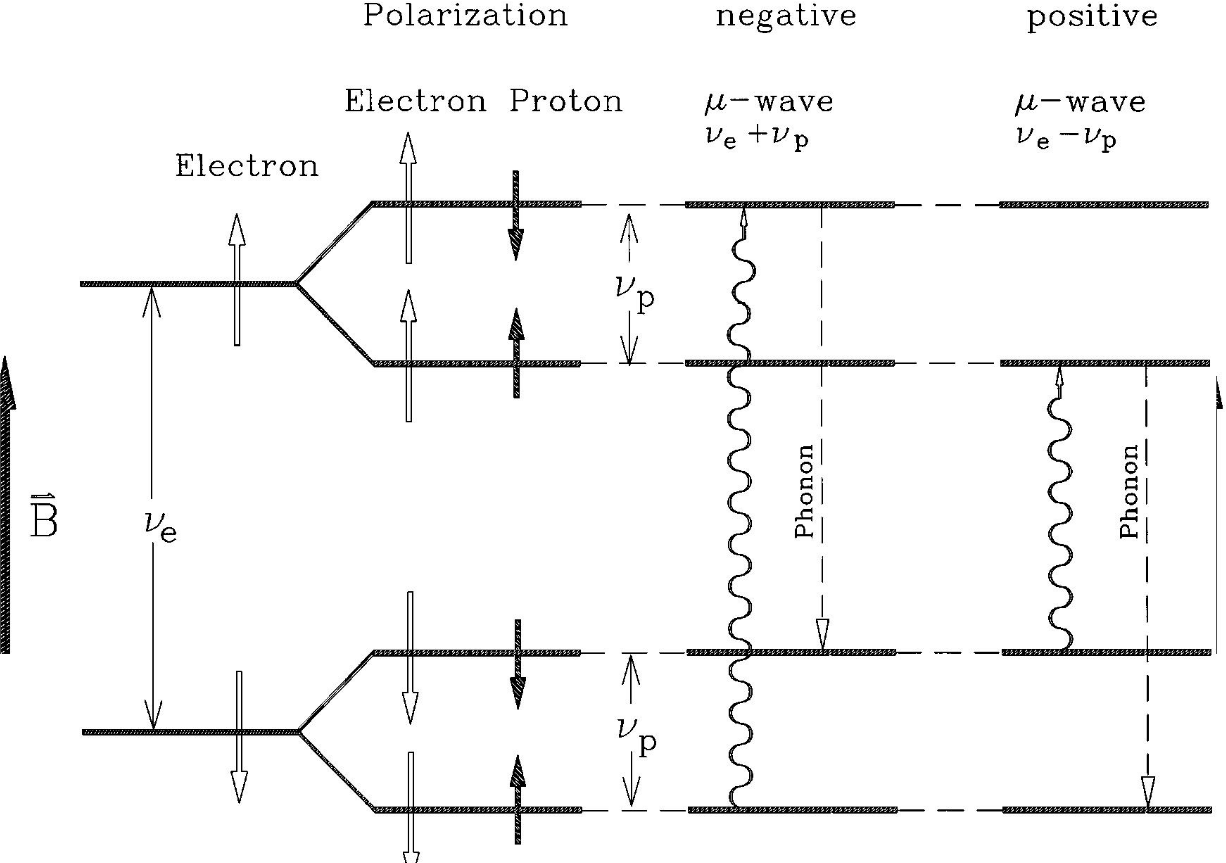
\includegraphics[scale=.25]{img/dnp.png}
 % dnp.png: 1226x863 pixel, 72dpi, 43.25x30.44 cm, bb=0 0 1226 863
 \caption{DNP diagram \cite{dnpdiagram}.  The white arrows are electron polarization and the black arrows are proton polarization.  Microwaves at a frequency difference $\nu_e\pm\nu_p$ flip the spins of both particles, and the electron's superior lattice coupling ensures it will flip back before the proton.}
 \label{fig:dnp-diagram}
\end{figure}


The microwave frequency can either be the sum of the proton and electron splitting frequency or the difference, depending on whether the nucleons are to be aligned with or against the magnetic field. 
\section{NMR}

Nuclear Magnetic Resonance (NMR) is the method we use to measure the polarization of the target material.  Essentially, a coil in the immediate vicinity of the target acts as the inductor in an LCR circuit, the inductance of which changes as a function of the magnetic susceptibility of the nuclei in the coil.  Since the magnetic susceptibility and polarization are related, the resonance frequency of the LCR circuit tell us information about the polarization of the target material\cite{qmeterbook}. 

\subsection{Liverpool Q-Meter}

\subsubsection{$\lambda$/2 Cable}

\subsubsection{Diode Detector}

\subsubsection{Phase Sensitive Detector and BRM}

\subsection{PDP}

\section{Frozen Spin} 
 
 The target is polarized in a 2.5 T field, called the polarizing field.  The target will lose all polarization in an environment free of magnetic field.  However, the detector cannot fit around the polarizing magnet, and the polarizing magnet would obstruct outcoming neutrons, anway).  To maintain polarization while the target is in the detector, an internal 0.5 T field is turned on inside the fridge and the polarizing magnetic is wound down and removed.  The 0.5 field, called the holding field, sufficiently maintains polarization of nucleons while the detector is moved aroud the target and data is taken.

\section{Refrigerator} 
Since the polarization goes like the inverse of temperature, colder environments make for better polarized targets.  In our case, we use a dilution refrigerator, one that mixes the two isotopes \het{} and \hef{} for cooling, to reach target temperatures below 0.1 K.

\subsection{\hef{}Cooling (Evaporator and Separator)}

\subsection{Dilution}

The dilution refrigerator principle relies on the splitting of a \het/\hef{} mixture into two distinct phases, a \het{} concentrated phase and a \het{} dilute phase.  The area labeled ``Two-phase region'' in Figure \ref{fig:dilutiondiagram} illustrates which mixtures, characterized by \het{} concentration, are inaccessible at which temperatures.  Since two distinct phases in thermal contact are always in or striving for thermodynamic equilibrium, changing the concentration of the dilute phase (by pumping \het{} out of it) will cause atoms from the concentrated phase to cross the phase boundary to restore balance.  Since the heat change of mixing (enthalpy difference between the dilute phase and concentrated phase) is positive, the \het{} crossing the phase boundary must absorb energy from the surrounding environment, which it does in the form of heat.\cite{hocktechniques}

\begin{figure}
 \centering
 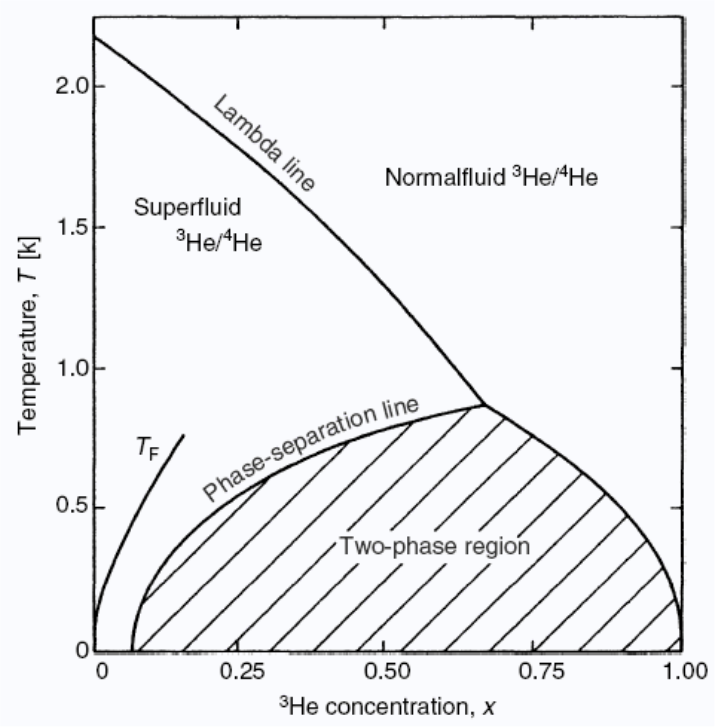
\includegraphics[scale=.45]{img/dilutiondiagram.png}
 % dilutiondiagram.png: 715x727 pixel, 72dpi, 25.22x25.64 cm, bb=0 0 715 727
 \caption{The famous diagram that shows the splitting of two distinct phases of $\het$-$\hef$ mixture. \cite{dilutiondiagram}}
 \label{fig:dilutiondiagram}
\end{figure}
 



\chapter{Hardware}
\label{hardware}
This chapter is an index and a catalog of all the equipment used in the project.
 
\section{Fridge}
  \subsection{Assembly Tools}
\subsubsection{OVC}

\begin{itemize}
  \item wire gripping pliers
  \item 5 mm allen key
  \item tee pilot pins  
\end{itemize}

\subsubsection{IVC}
\begin{itemize}
  \item solder station
  \item 2.5 mm allen key
  \item indium waste box
  \item wooden or hard plastic q-tips
  \item wire cutting pliers
  \item isopropyl alcohol 
\end{itemize}

\subsubsection{Microwave guide support}

\begin{itemize}
  \item flat head screwdriver
  \item fine tip squeeze-to-open tweezers 
\end{itemize}
 
\subsubsection{Mixing chamber}

\begin{itemize}
  \item mixing chamber customized open wrench
  \item 1.5 mm allen key
  \item indium waste box
  \item wooden or hard plastic q-tips
  \item wire cutting pliers
  \item isopropyl alcohol 
\end{itemize}


  \subsection{Cryogenic Instruments}

\subsubsection{\hef{} sensors}
  \begin{itemize}
   \item 2x \textit{Lake Shore\circledR} DT-670 silicon diode
\item \textit{Lake Shore\circledR} PT-102 platinum RTD
\item \textit{Lake Shore\circledR} Quad-Lead cryogenic wire, 36 AWG
  \end{itemize}
\subsubsection{\het{} sensors}
\begin{itemize}
 \item \textit{Lake Shore\circledR} DT-670 silicon diode
 \item \textit{Omega\circledR} KHLV-0502 Kapton heater
 \item \textit{Lake Shore\circledR} RX-202A-AA ruthenium oxide sensor
 \item \textit{Lake Shore\circledR} GR-200A-30 germanium diode
 \item 4-wire Matsushita resistor (model unknown) 

\end{itemize}

  \subsection{Magnet Leads}
\begin{itemize}
 \item OFHC copper leads
\item insulating mylar
\item Kapton tape
\item small flat head screwdriver
\item minature flat head screws
\item \textit{Solid Sealing\circledR} KT20678 copper conductor KF feedthrough
\end{itemize}


\section{Target Material}
\begin{itemize}
 \item cryogenic storage \lnn{} dewar
\item open styrofoam tub, about 5-10 liters
\item tweezers
\item hemostats
\item \lnn{} transfer dewar
\item cryogenic gloves
\end{itemize}

\section{Fridge Stand Mounting/Swinging Tools}

\begin{itemize}
  \item 13 mm combination wrench
  \item long-shaft 3/16\inches{} ball driver
  \item 10 mm combination wrench
  \item 5 mm allen key
  \item fridge lever
  \item \textit{80/20$^\circledR$} 5/16\inches{}-18 nuts, bolts
\end{itemize}


\section{Pump Station Area}
  \begin{itemize}
   \item Alcatel or VIC leak checker
   \item KF-25 plastic blank off
   \item KF-25 flexible hose
  \end{itemize}

  \subsection{\het{} Pumps} %use \hef{} to put space after newcommand
  \subsection{\hef{} Pumps}
  \subsection{\lnn{} Trap}
\begin{itemize}
 \item \lnn transfer dewar
\item cryogenic gloves
\item heat gun
\end{itemize}

  \subsection{Helium Gas Cylinders}

  
\section{Vault Pumps}
  \subsection{OVC}
  \subsection{IVC}

\section{Cryogenics}
  \subsection{Safety}
  \subsection{Transfer Lines}

\section{Vault Electronics Rack}
  \subsection{Patch Panel}
  \subsection{}

\section{NMR}

\section{Microwaves}
\chapter{Safety} 
\label{safety}
This chapter is about personnel safety, not equipment safety.  Learning to use HiFrost equipment properly without damaging anything is the aim this whole manual.  Safety of lab users, however, is important enough to warrant an entire devoted chapter, even if many points are reiterated throughout the document.

\vspace{1cm}
\fbox{\parbox{.93\textwidth}{\subsubsection{Ways to die or become seriously injured working on HiFrost:}
\begin{itemize}
\item Cryogenic explosions
\item Cryogenic burns
\item Oxygen depravation
\item Electric shock
\item Falling
\item Hot surfaces
\item Chemical exposure
\end{itemize}
}}

\section{Cryogenic Safety}
Both liquid nitrogen (\lnn, 77 K) and liquid helium (LHe, 4 K) are used during HiFrost operation.  The two primary cryogenic safety concerns are over-pressurization (explosion) of cryogenic vessels and cryogenic burns.  \lnn{} and LHe are each at risk of both, and precautions are taken while handling either. 
\subsection{Equipment}
\subsubsection{Cryogenic gloves}
Cryogenic gloves are lined internally with super-insulation and are long enough to cover past halfway between the wrist and elbow.  HiFrost equipment includes large and medium sized sets of gloves, and the best fitting size should always be used.  Typical activities requiring use of cryo gloves are filling the \lnn{} trap, inserting and removing LHe transfer lines, filling \lnn{} dewars for the target loading procedure, and making or manipulating target beads.

\subsubsection{Goggles}
Wearing googles and/or a face shield while handling open \lnn{} dewars is recommended.  Goggles also protect users in the vicinity of the large helium gas plumes expected during LHe dewar filling procedures.

\subsubsection{Closed toed shoes}
The general FEL safety regulations preclude anyone from wearing open toed shoes in controlled areas.  Still, there are areas outside the radiation perimeter where cryogens may be handled (e.g., the supply dewar just outside the bay doors), and closed toed shoes must be worn when handling \lnn{} or LHe vessels.
 
\subsection{Cryogenic Explosions}
The principle hazard of handling cryogens is an explosion caused by an enclosed volume of liquid warming up without adequate pressure relief for the evaporated gas.  For this reason, every container that holds cryogenic liquid has a pressure relief valve, and most large dewars have a non-configurable, one time use emergency burst disk.  


An important exception to the pressure relief rule is the \het{} circuit in the dilution refrigerator and pumping system.  Due to the scarcity and cost of \het, it is unacceptable to install pressure relief valves venting to atmosphere.  Instead, a single internal pressure relief valve, which opens at about 1.2 bar, is installed on the \het gas rack and should open if the pressure in the circuit rises due to a plug.  The pressure relief valve can only open if the valves leading to the fridge (via the condensor and still lines) are opened in the appropriate configuration.  Failure to do this could lead to catastrophic damage to the pumping system or, worse yet, the refrigerator itself.  

\subsubsection{Three valves rule}

The 500LD, 100LD and most supply helium dewars have three pathways for helium to escape in addition to the burst disk.  The three pathways are:
\begin{enumerate}
\item the pressurization port, where external gas is applied to the dewar
\item a pressure relief valve, usually set around 2-4 PSI
\item the inlet/outlet pathways where transfer lines connect through the top of the dewar 
\end{enumerate}

In general, all three of these ports may have manual valves to prevent helium from flowing through them.  For example, at the end of a 500LD fill, we close the outlet port on the filling dewar to halt the transfer, and the pressure relief valve is already closed to maintain liquid flow to the 500LD (see Section \ref{practical-op:500LDfill}).  The pressurization valve is always closed unless specifically venting the dewar or actively applying pressure to it.  The three valves rule is

\vsepfbox{\parbox{.93\textwidth}{\centering
\textbf{At least one of the three pathways on a cryogenic vessel must be open at all times.}
}}

If all three pathways are closed simultaneously, the radiative heat load (present in all dewars) will warm up the trapped liquid, increasing the pressure on the dewar until the burst disk breaks.  If for whatever reason the emergency burst disk fails, the resulting pressure will lead to an enormous explosion, easily fatal to any personnel nearby \cite{lnexplosion}. 

\subsection{Cryogenic Burns}
Cryogenic burns may happen by touching a liquid cryogen or cold gas plume, touching a bulk mass that was recently cooled by cryogenic liquid, or inhaling cold gas.  Use cryogenic gloves whenever handling liquid cryogens or surfaces they have recently cooled (like transfer lines), and always wear closed toed shoes in the lab.


\vspace{1cm}
\fbox{\parbox{.92\textwidth}{\subsubsection{In the event of a cryogenic burn\cite{epling}:}
\begin{itemize}
\item If prehospital warming is attempted, options include placing the affected area in warm (not hot) water or warming it using body heat (eg, placing frostbitten fingers in the axillae).
\item  You can flushing the area with tepid water but, in order to avoid tissue damage, a forceful flow of water should NOT be used.
\item Never use dry heat.  Never apply direct heat.
\item  Do not rewarm frostbitten tissue if there is a possibility of refreezing before reaching definitive care. This would result in worse tissue damage.
\item Do not rub frostbitten areas in an attempt to rewarm them; this can cause further tissue damage.
\item Remove any clothing or jewelry that may restrict circulation to injured area. 
\item  Do not cover the area; leave injured area open to air.
\end{itemize}
}}
\vspace{1cm}

To get help\cite{epling}, call Duke Employee Occupational Health and Wellness Hotline, available at any time, for assistance with a typical burn, 919-684-8115.  A Duke Hospital Operator with answer and then will page the EOHW nurse to your number.  During business hours you may also call EOHW main number, 919-681-3136, option 2 and ask for nurse.  Call 911 if situation is life threatening.  Provide the following information\cite{epling}:

\begin{itemize}
\item Agent causing cryogenic burn
\item Skin tone/color (white, pale, red, or blue).
\item Presence of Blisters (yes or no)
\item Location and area of injury
\item Presence of open skin (yes or no)
\item Current treatments
\item Any additional past medical information, medications, allergies
\item Confirm that the area of liquid nitrogen or hydrogen is secure and safe
\end{itemize}

\section{Oxygen Depravation}

Work with cryogenics automatically involves an oxygen depravation hazardous (ODH) environment, because the contents any liquid cryogen vessel are capable of displacing many times its volume of breathable air.  Generally, liquid helium can displace 1 cubic meter of breathing air for each liter of liquid that is quickly boiled, meaning the 100 L HiFrost dewar can displace 100 cubic meters of air.  Additionally, helium is colorless, odorless and tasteless, so it is often impossible for a worker to tell when they are not getting enough oxygen until the symptoms of oxygen deprivation begin to kick in.

The following information and the content of Table \ref{fig:jlabodh} is taken from Thomas Jefferson National Lab's ODH manual. \cite{jlabodh}

\paragraph{Health Effects of Reduced Oxygen}

Normal air is approximately 21\% oxygen and 78\% nitrogen. The remaining 1\% is mostly argon. Health effects begin at an oxygen concentration of 17\%. Oxygen monitors at Jefferson Lab are set to alarm at 19.5\%. This advance warning should give ample time to escape the hazard area.  The early health effects are difficult to detect so the oxygen monitors are relied upon to give early warning:

\begin{figure}
\centering
\begin{tabular}{|c|p{6cm}|}
 \hline
Percent Oxygen & Health Effects \\
\hline
17 & night vision reduced \newline increased breathing volume \newline accelerated heartbeat \\
\hline
16 & dizziness \newline reaction time for new tasks is doubled\\
\hline
15 & poor judgement \newline poor coordination \newline abnormal fatigue upon exertion \newline loss of muscle control\\
\hline
10-12 & very fault judgement \newline very poor muscular coordination \newline loss of consciousness\\
\hline
8-10& nausea \newline vomiting \newline coma\\
\hline
$<$8 & Permanent brain damage \\
\hline
$<$6 & spasmodic breathing \newline convulsive movements \newline death in 5-8 minutes \\
\hline
\end{tabular} 
\caption{JLab ODH manual's list of health effects of oxygen deprivation.}
\label{fig:jlabodh}
\end{figure}

\section{High Voltage Safety}
\section{Gravity Safety}

No high places should be reached without the appropriate ladder during Hifrost operations or activities.  Remember the following 5 rules of ladder safety\cite{laddersafety-duke}:
\begin{enumerate}
 \item Choose the right ladder for the job.
 \item Inspect the ladder before you use it.
 \item Set up the ladder with care.
 \item Climb and descend ladders cautiously.
 \item Use safe practices when working on a ladder.
\end{enumerate}

Additional information ladder safety is provided by OSHA\cite{laddersafety-osha}.

\section{Magnetic Field Safety}

Aside from being full of 77 K liquid nitrogen and 4 K liquid helium, the polarizing magnet poses a safety threat by virtue of its 2.5 T field.  The 0.5 T frozen spin field is considerably weaker and, due to its localization inside the radiation shield of the fridge, less accessible to personnel and foreign objects.

The most likely danger is a ferromagnetic object (like a wrench) striking personnel as it is pulled towards the polarizing magnet\cite{magnetsafety}.  The best safety measure against this is making sure Hifrost workers and anyone else in the GV know when the magnet is on and do not keep loose ferromagnetic objects on their person.

Anyone with an implanted medical device, such as a pacemaker, should alert Hifrost officials before working on or near Hifrost equipment during a polarizing magnet cooldown.  Under no circumstances should they get closer than the 10 gauss line while the magnet is energized without speaking with their physician and the director of DFELL\cite{pacemakersafety}.

The EIO has a strong enough magnetic field to pull a ferromagnetic object in from a few inches away, so care should be taken to not allow any loose tools to smash into it.

\section{Chemical Safety}
\subsection{Heavy elements}
\subsubsection{Indium}
Indium is used for sealing two interfacing sets of flanges in the dilution refrigerator.  Disassembling the refrigerator necessarily entails scraping indium off these flanges, and assembling the fridge requires cutting and setting the seal from a roll of indium wire.

While no cases of indium poisoning by oral consumption have been recorded, it remains a heavy element and toxic to humans if it enters the blood stream.  As a precaution, wearing latex gloves is recommended while handling indium, and hands should be washed immediately after, especially before taking a lunch break or leaving for the day.

\subsubsection{Lead}
Lead is a toxic metal often used in the laboratory due to its density and availability.  Inorganic lead is not readily absorbed through the skin, but once it enters the body (through ingestion or inhalation) it is carried by the bloodstream to the ``bone, teeth, liver, lungs, kidneys, brain and spleen'' in high concentrations \cite{aafp98}.  Children and pregnant women are particularly at risk to damage from lead poisoning \cite{epa13}


Lead bricks are used at the University of Virginia PTGroup lab to counter the weight of the fridge on the stand.  Lead bricks are also present at HIGS around the beam line and UTR, although they are not usually found in the Vault.  Work gloves and hard-toed shoes are recommended when carrying or lifting lead bricks.  Any skin that was exposed to lead bricks or lead dust should be washed immediately after performing duties requiring lead exposure.

\subsection{Isopropyl Alcohol}
Isopropyl alcohol is used to clean the indium and KF-oring surfaces on the fridge and in the pumping system.  It is generally safe to be exposed to, but if there is a large quantity in an open container (like a bath for soaking vacuum parts) make sure the area is well ventilated and anyone working nearby knows about it.  Symptoms of isopropyl alcohol inhalation are dizziness, drowsiness and headache, and may cause unconsciousness \cite{isopropmsds}. 

Isopropyl alcohol has a flash point (the lowest temperature it emits ignitable fumes) of 53$^\circ$ F, and care should be taken not to expose alcohol bottles to open flames.
\chapter{Practical Operation} 
\label{chapter:practical-op}
\begin{figure}[!h]
 \centering
 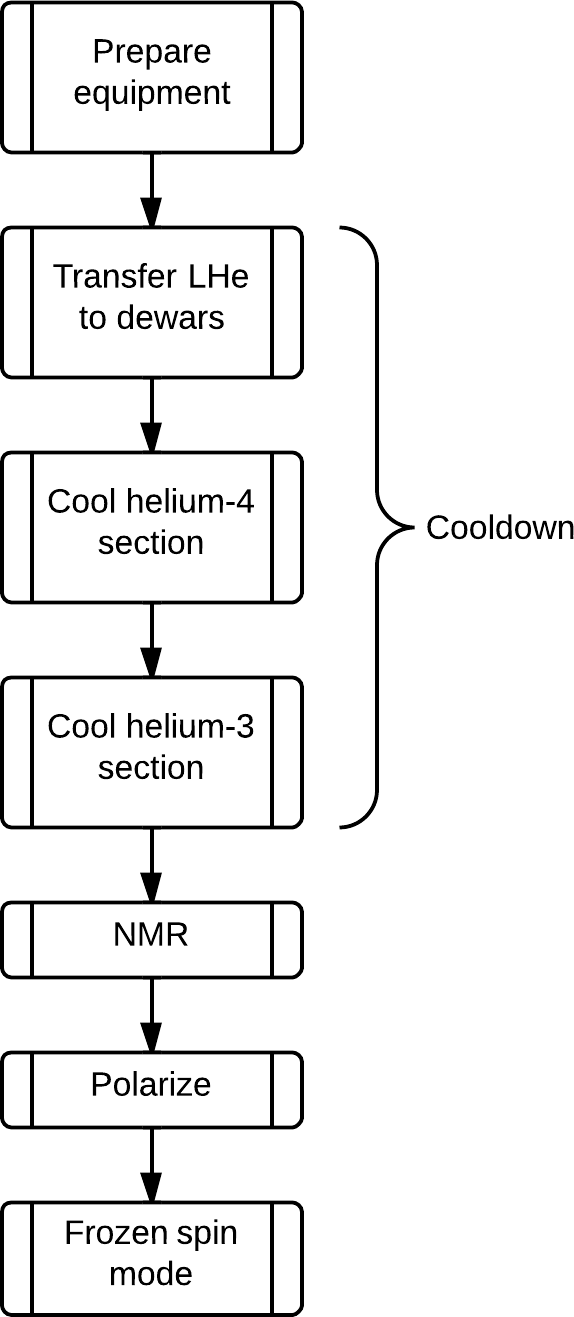
\includegraphics[scale=.24]{./img/cooldown-overview-flowchart.png}
 % cooldown-overview-flowchart.png: 102x490 pixel, 100dpi, 2.59x12.45 cm, bb=0 0 73 353
 \caption{Practical steps to polarize target material with HiFrost.}
 \label{fig:cooldown-overview-flowchart}
\end{figure}

This chapter assumes the reader is familiar with everything safety related.  Read Chapter \ref{safety} before attempting anything here.



\section{Cooldown}
\subsection{Prep}
\label{practical-op:prep}
Go down the checklist found in Appendix \ref{appendix:checklist-for-cooldown}, reporting any issues to the senior cooldown scientist.

\textbf{This step is not optional}: the rest of this operational procedure assumes all prep work is successfully completed and equipment bugs are worked out.  See walkthroughs for specifics tasks in Chapter \ref{procedures}.

\section{LHe Transfer Overview}

Figure \ref{fig:cryo-schematic-all} is a schematic of the LHe transfer system.  More detailed figures of the dewars are found later in the chapter, and complete technical drawings of the TLs are found in Appendix \ref{appendix:tl-drawings}.

\begin{figure}[htbp!]
 \centering
 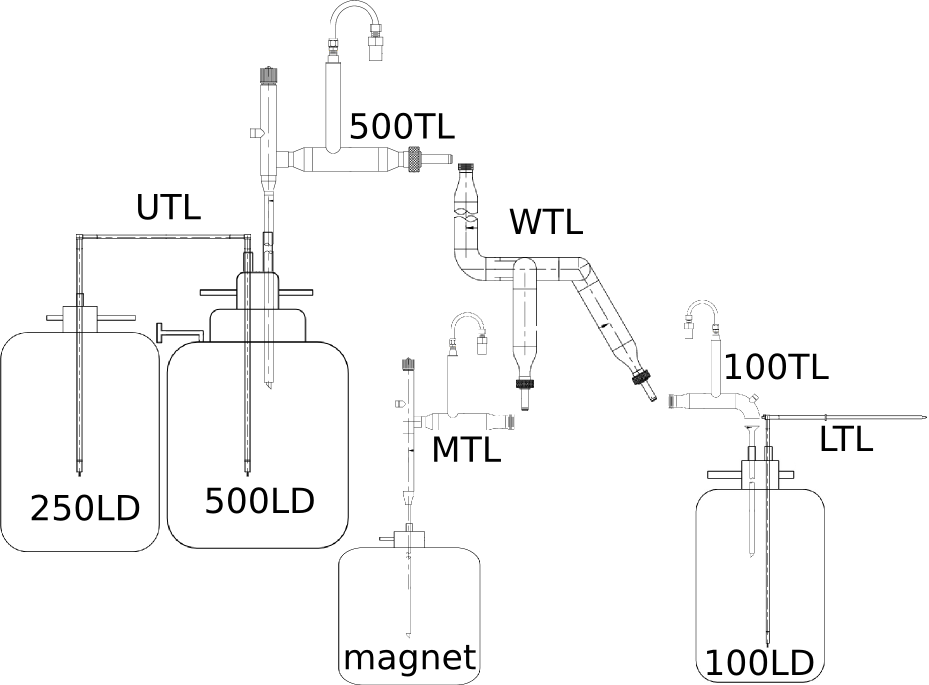
\includegraphics[width=\textwidth]{./img/cryo-schematic-all.png}
 % cryo-schematic-all.png: 0x0 pixel, 0dpi, 0.00x0.00 cm, bb=
 \caption{Schematic overview of the LHe transfer and storage system.}
 \label{fig:cryo-schematic-all}
\end{figure}


\subsection{Dewar Filling}
The 500LD and 100LD are initally filled before cooling the fridge.  The magnet is filled either before or after dilution.

The 250LD has an LHe outlet port, a pressurization/exhaust port and the pressure relief port, shown in Figure \ref{fig:250LD-cartoon}.  Each port has an accompanying valve.

The 500LD has an inlet port (for LHe filling and the level probe), an outlet port, a pressurization port, a vacuum pump out port and a pressure relief port, as shown in Figure \ref{fig:500LD-cartoon}.  Only the pressurization, vacuum pump out and pressure relief ports have accompanying valves.


\begin{figure}[!htbp]
\centering
 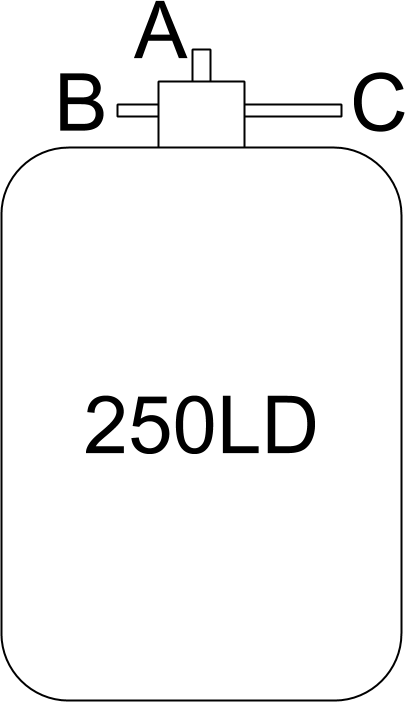
\includegraphics[width=.25\textwidth]{./img/250LD-cartoon.png}
 % 500LD-cartoon.pdf: 0x0 pixel, 0dpi, nanxnan cm, bb=
 \caption{An example of 250LD ports: A) LHe outlet port, B) pressure relief valve, C) pressurization/exhaust port.}
 \label{fig:250LD-cartoon}
\end{figure}


\begin{figure}[!htbp]
 \centering
 \begin{minipage}{.35\textwidth}
 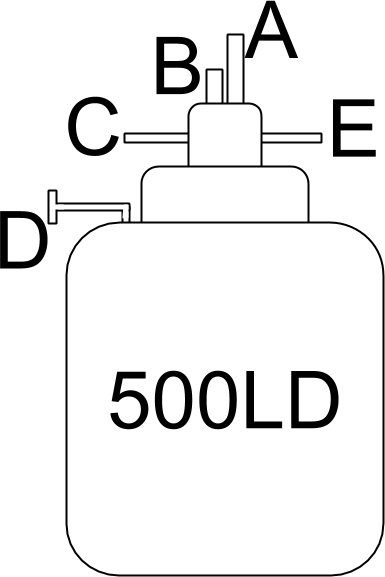
\includegraphics[width=\textwidth]{./img/500LD-cartoon.png}
 % 500LD-cartoon.pdf: 0x0 pixel, 0dpi, nanxnan cm, bb=
 \caption{The 500LD ports.}
 \label{fig:500LD-cartoon}
 \end{minipage}
 \quad
  \begin{minipage}{.50\textwidth}
 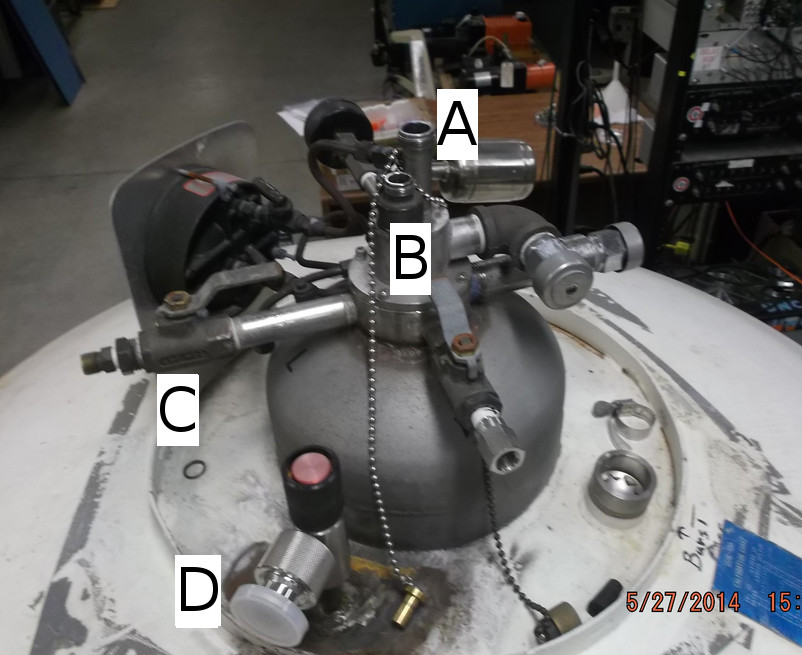
\includegraphics[width=\textwidth]{./img/500LD-photo.jpg}
 % 500LD-cartoon.pdf: 0x0 pixel, 0dpi, nanxnan cm, bb=
 \caption{Photo of 500LD: A) LHe inlet port, B) LHe outlet port, C) pressurization port, D) vacuum pump out port, E) pressure relief valve.}
 \label{fig:500LD-photo}
 \end{minipage}
 \end{figure}




\subsubsection{500LD Fill}
\label{practical-op:500LDfill}
\begin{enumerate}
 \item Weigh a full 250LD according to the procedure in Section \ref{weigh-250LD} before breaking the seal on it.
 \item Check 250LD level using the procedure in Section \ref{procedure:check-lhe-level}.
 \item Place correct Goddard fittings on the 250LD and/or the UTL.
 \item Blow out UTL with helium gas by fitting the universal hose over it and putting about 2 PSI on the helium cylinder. \label{procedure:500LDfill-blowoutUTL}
 \item $[$\textbf{initial 500LD fill only}$]$ Purge the 500LD with helium gas by hooking up the pressurization line, closing the main flow valve, opening the pressure release valve and putting 5 pounds of pressure on the 500LD for about 10 minutes (Figure \ref{fig:500LDfill-02-blow-out-500LD}).  Remove the pressurization line. \label{procedure:500LDfill-purge500LD}%for some godforsaken reason square brackets have to be in math mode to not ruin enumerated lists
 \item Open main flow valve on 500LD to vent pressure (if any), then open pressurization valve making sure the pressurization port is not pointed at anyone.
 \item Release the 250LD pressure from the main flow valve and close the pressure relief valve.  Slowly lower the correct end of the UTL down into the 250LD about 30 cm or until helium gas is blowing out the 500LD end, as shown in the left side of Figure \ref{fig:500LDfill-03-04-insert-UTL-in-250LD-and-500LD}.  Then, lower the 500LD end in as far as it can go, while continuing to slowly lower the 250LD side at a rate of about 2 cm/s.  A cold plume should be coming out of the 500LD.  Check that no gas is escaping through the Goddard fittings on either dewar (if it is, replace fitting o-rings). \label{procedure:insert-UTL-in-250LD}
 \item Hook up the pressurization line to the 250LD pressurization port using the procedure in Section \ref{procedure:attach-pressurization-line} and open the pressurization valve as shown in the right side of Figure \ref{fig:500LDfill-03-04-insert-UTL-in-250LD-and-500LD}.  There should now be 2 PSI on the 250LD. \label{procedure:insert-UTL-in-500LD}
 \item Periodically measure the 250LD level using the procedure in Section \ref{procedure:check-lhe-level}.  When it is empty, stop flow from the pressurization cylinder regulator and disconnect the pressurization line.
 \item Simultaneously raise both sides of the UTL out of the dewars and hang it on the wall to warm up.
 \item Bung the 500LD inlet port, close the 500LD pressurization valve, and leave open the pressure relief valve.
 \item On the 250LD, open the pressure release valve and close the main flow and pressurization valves.
 \item Recover the Goddard fittings from the 250LD and bring it back to the weigh area.  Record the final weight on the log sheet.
\end{enumerate}

\begin{figure}[htbp!]
 \centering
 \begin{minipage}{.47\textwidth}
 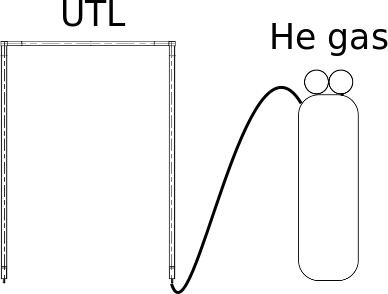
\includegraphics[width=\textwidth]{./img/500LDfill-01-blow-out-UTL.png}
 \caption{Blowing out the UTL with He gas (Step \ref{procedure:500LDfill-blowoutUTL}).}
 \label{fig:500LDfill-01-blow-out-UTL}
 \end{minipage}
 \quad
 \begin{minipage}{.47\textwidth}
 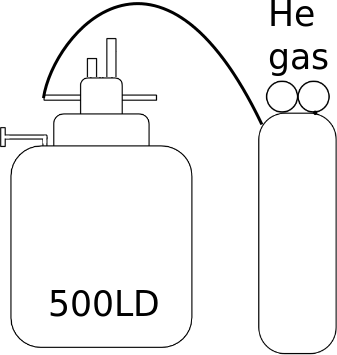
\includegraphics[width=\textwidth]{./img/500LDfill-02-blow-out-500LD.png}
 \caption{\textbf{Initial 500LD fill}, purging the 500LD with He gas (Step \ref{procedure:500LDfill-purge500LD}).}
 \label{fig:500LDfill-02-blow-out-500LD}
 \end{minipage}
\end{figure}

\begin{figure}[htbp!]
 \begin{minipage}{.38\textwidth}
 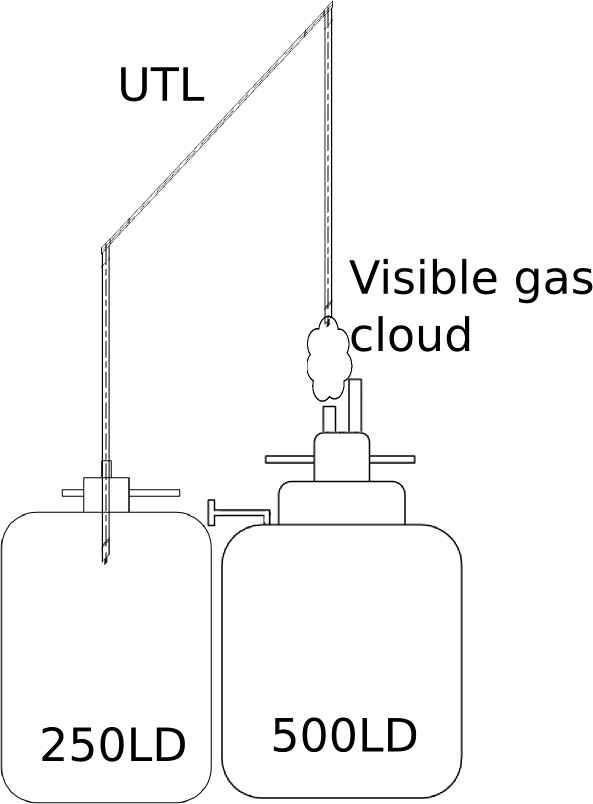
\includegraphics[width=\textwidth]{./img/500LDfill-03-insert-UTL-in-250LD.png}
 \end{minipage}
  \quad
 \begin{minipage}{.58\textwidth}
 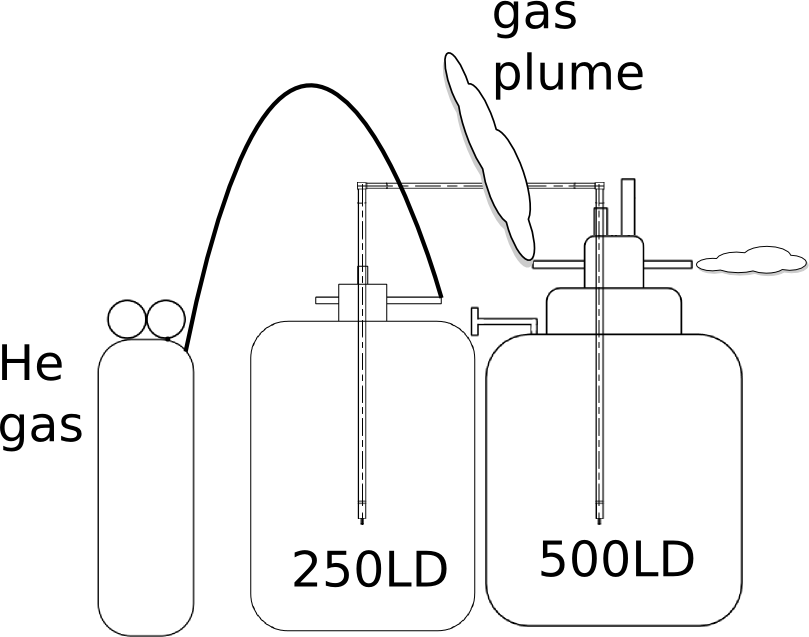
\includegraphics[width=\textwidth]{./img/500LDfill-04-insert-UTL-in-500LD.png}
 \end{minipage}
 \caption{Inserting the UTL first in the 250LD, then the 500LD, as described in Steps \ref{procedure:insert-UTL-in-250LD} and \ref{procedure:insert-UTL-in-500LD}.  The pressurization line is attached to the 250LD to facilitate liquid transfer.}
 \label{fig:500LDfill-03-04-insert-UTL-in-250LD-and-500LD}
 \end{figure}
 


\subsubsection{Initial 100LD Fill}

The 100LD has an entrance port, a main flow port, an exhaust port and a pressure relief port.  The exhaust and pressure relief ports have accompanying valves.
 
 \begin{figure}[!htbp]
 \centering
 \begin{minipage}{.55\textwidth}
 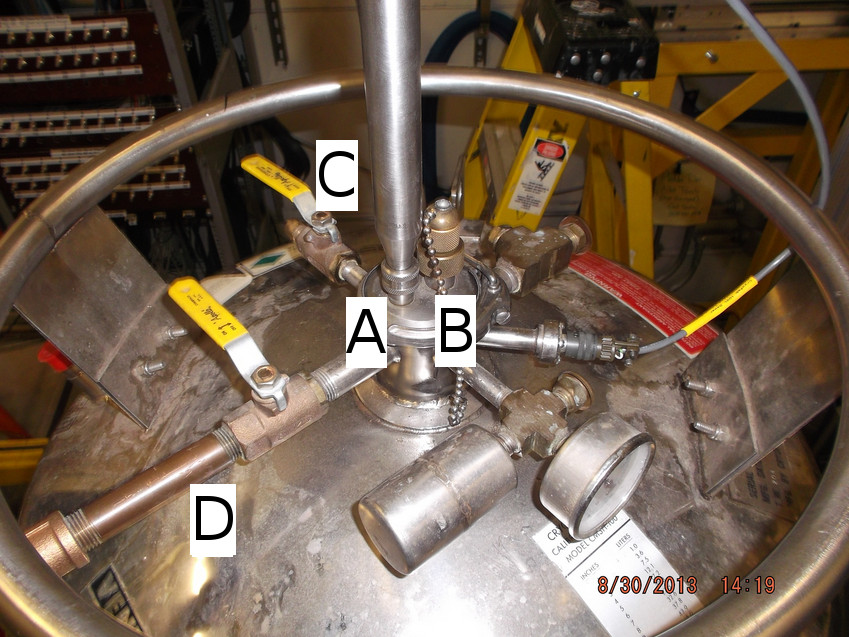
\includegraphics[width=\textwidth]{./img/100LD-photo.jpg}
 % 500LD-cartoon.pdf: 0x0 pixel, 0dpi, nanxnan cm, bb=
 \caption{Photo of 100LD: A) LHe inlet port, B) LHe outlet port, C) pressure relief valve, D) pressurization/exhaust port.}
 \label{fig:100LD-photo}
 \end{minipage}
 \quad
  \begin{minipage}{.40\textwidth}
 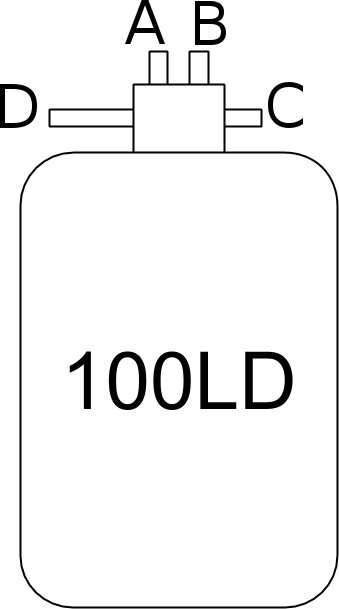
\includegraphics[width=\textwidth]{./img/100LD-cartoon.jpg}
 % 500LD-cartoon.pdf: 0x0 pixel, 0dpi, nanxnan cm, bb=
 \caption{100LD cartoon.}
 \label{fig:100LD-cartoon}
 \end{minipage}
 \quad
\end{figure}

\begin{enumerate}
 \item Purge the 500TL with helium gas.  Make sure the flow valve is open.
 \item Make sure the correct Goddard fittings are on the 500LD and/or 500TL.
 \item Install the 100TL in the 100LD and attach the bayonet to the WTL.
 \item Close the magnet LHe inlet valve on the WTL (blue valve).
 \item Open the 100LD exhaust valve, close the pressure release valve and bung the main flow valve.
 \item Remove the bung from the WTL by the pump station area.
 \item Hook up the helium gas line in the GV to the 100LD exhaust port and pressurize to 2 PSI.
 \item Verify there is a positive pressure on the WTL by the pump station.  Increase the helium cylinder pressure if necessary.  Wait 10 minutes for the 100LD, 100TL and WTL to purge.
 \item Close the 500TL flow valve and stop purging it.
 \item Vent the 500LD through the pressurization port.
 \item Open the 500LD main flow port.
 \item Close the 500LD pressurization and pressure relief valves.
 \item Slowly lower the 500TL about 30 cm until helium gas starts flowing out.  It may need to go further in first, depending on how full the 500LD is.
 \item Watch the gas plume coming out of the end of the 500TL.  Slowly lower the 500TL in the 500LD at a rate of 1cm/s until the plume looks like a blowtorch, then immediately insert into the WTL and tighten.
 \item \textbf{Immediately remove the pressurization line from the 100LD exhaust port and open the 100LD pressure relief valve.} Verify gas is coming out the exhaust and make sure the exhaust is pointing towards the center of the room and not at personnel (the plume will quickly grow).
 \item Slowly lower the 500TL all the way down into the 500LD and tighten the Goddard fitting.  Use the heat gun if the Goddard fitting freezes before the 500TL is completely in.
 \item Hook up the pressurization line to the 500LD pressurization port using the procedure in Section \ref{procedure:attach-pressurization-line} and open the 500LD pressurization valve.
 \item Turn on the 100LD level probe and watch the monitor for the level to increase.
 \item When the 100LD is full there will be a large white plume coming from the exhaust and the level probe will read around 24.9 (arbitrary units). Close the 500LD pressurization valve and remove the pressurization line.  Then vent the 500LD through the pressurization port and open the 500LD pressure relief valve.
 \item Close the 500TL flow valve.
 \item Close the 100LD exhaust valve.
\end{enumerate}

\subsubsection{100LD Fill During Run}

\begin{enumerate}
 
 \item Verify the 500LD is full enough to top off the 100LD.  If not see above 500LD fill procedure.
 \item Set the regulator on the helium pressurization cylinder to 2 PSI.
 \item Open the 100LD exhaust valve and make sure the exhaust port is safely facing the center of the room.
 \item Hook up the pressurization line to the 500LD pressurization port using the procedure in Section \ref{procedure:attach-pressurization-line}.
 \item Open the main flow valve on the 500TL, then close the 500LD pressure relief valve.
 \item Open the 500LD pressurization valve.
 \item Verify the 100LD Goddard Fittings are not leaking gas.  If they do, remove the pressurization from the 500LD and close the 500TL main flow valve immediately.  Consult a high ranking lab official.
 \item When the 100LD is full, remove the pressurization from the 500LD, open the 500LD pressure relief valve and close the 500TL main flow valve.
 
\end{enumerate}


\subsection{Cool \hef{} Section}

When the 100LD is full, the fridge has been backfilled with helium gas and the rest of the system is ready for a cooldown, the LTL is inserted into the 100LD and fridge.  The separator pumps on the fridge are started and the pressure difference is enough to pull helium from the 100LD (no dewar pressurization needed).

The LHe travels through the LTL into the separator, which collects liquid while rejecting gas.  The gas is pulled out through two lines, the ``separator'' line which precools the \het{} inlet, and the shield line which provides a heat shink for the radiation shield.

When the separator is full, control valve 1 (CV1) allows helium to flow to the evaporator and control valve 2 (CV2) directs LHe to the holding magnet and IVC can.  CV2 is also used to quickly cool the MC when target material is at risk of thermal damaged.

The evaporator can hold LHe at 4K, but evaporator pumps are run to lower the helium vapor pressure and lower the temperature down to a minimum of about 1K.

\subsubsection{Insert LTL}
\begin{enumerate}
 \item See Section \ref{practical-op:prep} to make sure the fridge is ready to take LHe.
 \item Check the 100LD level probe and top off if necessary (see directions above).
 \item Blow out LTL with helium gas.
 \item Make sure 100LD can roll out from under the fridge stand area (so the LTL can be inserted), back under the fridge stand area, and then up to the fridge.  The IVC pump cart may have to be shifted around.
 \item Put 4 PSI on the fridge via the following steps: adjust the helium gas regulator to 4 PSI, open the valves between the regulator and the separator manifold, close all other separator manifold valves (so gas does not flow to separator pumps).
 \item Remove the LHe inlet bung and KF clamp from the fridge and verify the positive pressure from the separator.
 \item Stop purging LTL with gas and place a rubber in the fridge side.
 \item Remove bung from 100LD main flow port and slowly insert the LTL until it lines up with the fridge.
 \item Roll the 100LD in place under the fridge stand.
 \item Remove the LTL bung and wait for the gas plume to look like a blue torch flame, then roll the 100LD towards the fridge until the LTL is fully inserted and tighten the KF clamp around the LTL-fridge inlet joint.
 \end{enumerate}
 
 \begin{enumerate}
 \item Open CV1 and CV2 about 2 turns each.
 \item Immediately turn off the pressurization from the helium cylinder and turn on the separator pumps.  Open all valves between the separator pumps and the fridge, including bypass valves.  Pump on shield at max flow for 30 minutes and separator for 15 minutes\cite{tapio-cooldown-procedure}.
 \item Separator flow is only kept high when there is no liquid in the separator yet; thereafter control the shield flow keeping it below 20 mmol/s and reduce the separator flow to 5 mmol/s (see Appendex \ref{appendix:slpm-conversion} for flow conversion). 
 \item TODO Cooldown diverges from June 2014 cooldown at this point; consider separate document
\end{enumerate}


\subsection{Cool \het{} Section}
\subsection{Dilution}

\section{Polarization}

\section{NMR}

\section{Frozen Spin}
\blindtext

\chapter{Procedures} 
\label{procedures}  
\section{Evacuating Transfer lines}

\subsection{Cryofab TLs}

\subsection{LTL}

\section{Indium Extrusion}

\section{Making/Breaking Indium Seals}

\section{Magnet Lead Installation}

\section{Mounting Fridge}

\section{Dismounting Fridge}

\section{Cleaning Viton/Buna O-rings}

\section{Changing Kenol Connectors}

\section{Installing Heating Tapes}

\section{Purging Helium Lines}

\section{Vacuum Rise Testing}

\section{Stripping Fridge}

\section{Assembling Fridge}

  \subsection{MC}
  \subsection{Microwave Guide Support}
  \subsection{IVC}
  \subsection{OVC}

\section{Removing/Replacing \het{} Baffles} 
%-----subsystems.tex
\chapter{Subsystems}
\section{Thermistor Switch and Display}
The thermistor system is set up to provide signals from all of the thermistors to the USB-1608G data acquisition (DAQ) unit (and so be visible and recorded outside the vault), and to maintain the ability to put any of the thermistor readings on a display while in the vault.

The EIO Body thermistor is wired to a dedicated single channel controller, which displays the temperature, has a normally-closed relay with a high-temperature trip point (set to 40 $^\circ$C right now) in the Cober power supply interlock loop, and provides a DC voltage proportional to temperature to the DAQ (0 to 10 V corresponds to 0 to 100 $^\circ$C).

Three other thermistors (EIO water flow out, Q-meter P and Q-meter D) are wired to the thermistor switch panels. These are wired in series, and a 100 $\mu$A power supply runs current through these, and DAQ channels are wired in parallel with each of the thermistor wires. The signal is proportional to thermistor resistance.  These are 10 k$\Omega$ (at 25 $^\circ$C) NTC thermistors, so the signal is 1 volt at 25 $^\circ$C. A look-up table will need to be used to convert the readings to temperature.

The switch has 6 positions; Spare 1, EIO Flow, Q-meter P, Q-meter D, Spare 5 and Display Nothing. Set the switch to the thermistor which should be put on the display. When the switch is set to one of the first 5 positions, relays divert that thermistor signal to the display, and connect a short into the 100 $\mu$A PS loop. So, when you look at, say, EIO Flow, the DAQ signal for that channel will be zero volts, and that thermistor's temperature will show on the display. If the switch is set to Display Nothing, all 5 signals go the the DAQ. There is a 29.4 k$\Omega$ resistor for the display in the Display Nothing position, which displays as 0 $^\circ$C (or maybe 0.1).

The Spare 1 and Spare 5 positions also have 29.4 k$\Omega$ resistors, so the display will show zero on those positions as well, and the DAQ will get a pretty constant 2.94 V signal from them. These resistors can be replaced by thermistors in the future should the need for more temperature readings arise.

Referring to the schematic drawing, the switch is 4-Pole 6-Position (4P-6T).  Two poles are used to energize the selected relay by sending 24 VDC and 24 Common to the selected coil.

In the not-energized state, each relay connects the thermistor for that channel to the 100 $\mu$A power supply.  Each thermistor is also wired to a DAQ channel.  The thermistors are wired in series, so the same 100 $\mu$A flows through all thermistors.

In the energized state, each relay connects the thermistor for that channel to the other two poles of the 4P-6T switch, which connects this thermistor to the thermistor display on the panel.  Also, the thermistor is replaced by a short circuit so the 100 $\mu$A will continue to flow through the rest of the thermistors.

Also seen is a schematic, Figure \ref{fig:subsystem-thermistor-schematic}, for the 100 $\mu$A power supply, which is based on a $\mu$A723 voltage regulator.  Operating with a 24 VDC V$_{\textrm{cc}}$ supply, the power supply output can provide 100 $\mu$A through a load of 0 to 100 k$\Omega$.

The 6 photos, Figure \ref{fig:subsystem-thermistor-photos}, show the front and back of the three small panels which comprise the thermistor system – Switch panel, Display panel, and Relay panel.  The Switch panel and Relay panel are connected with a 25 wire DB-25 cable.  The display panel also holds a flow switch display which is wired to the EIO cooling water flow switch.

\begin{figure}[!htbp]
 \centering
 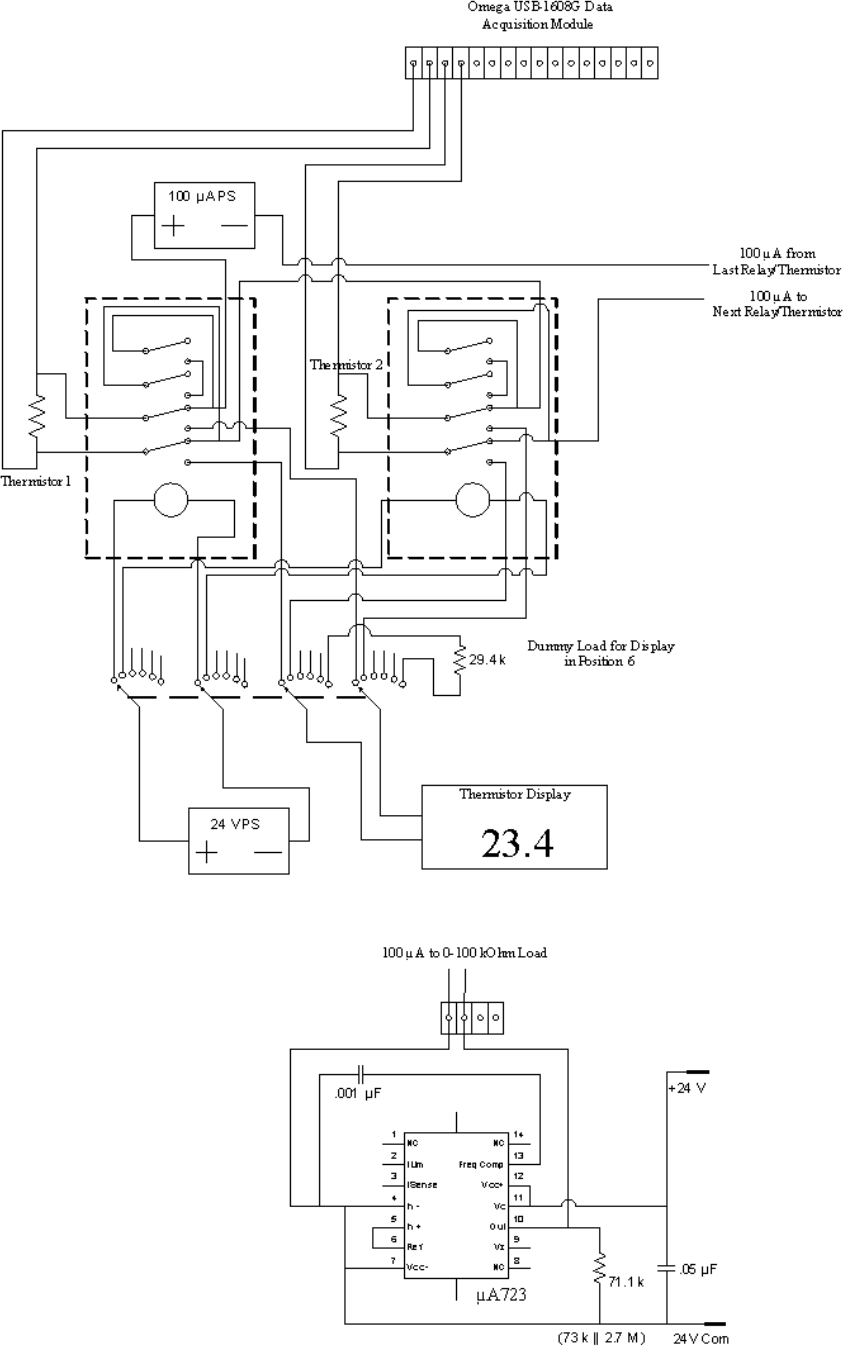
\includegraphics[height=.9\textheight]{./img/subsystem-thermistor-schematic.png}
 % subsystem-thermistor-schematic.png: 0x0 pixel, 2870220dpi, 0.00x0.00 cm, bb=
 \caption{Schematic of thermistor system.}
 \label{fig:subsystem-thermistor-schematic}
\end{figure}
\begin{figure}[!htbp]
 \centering
 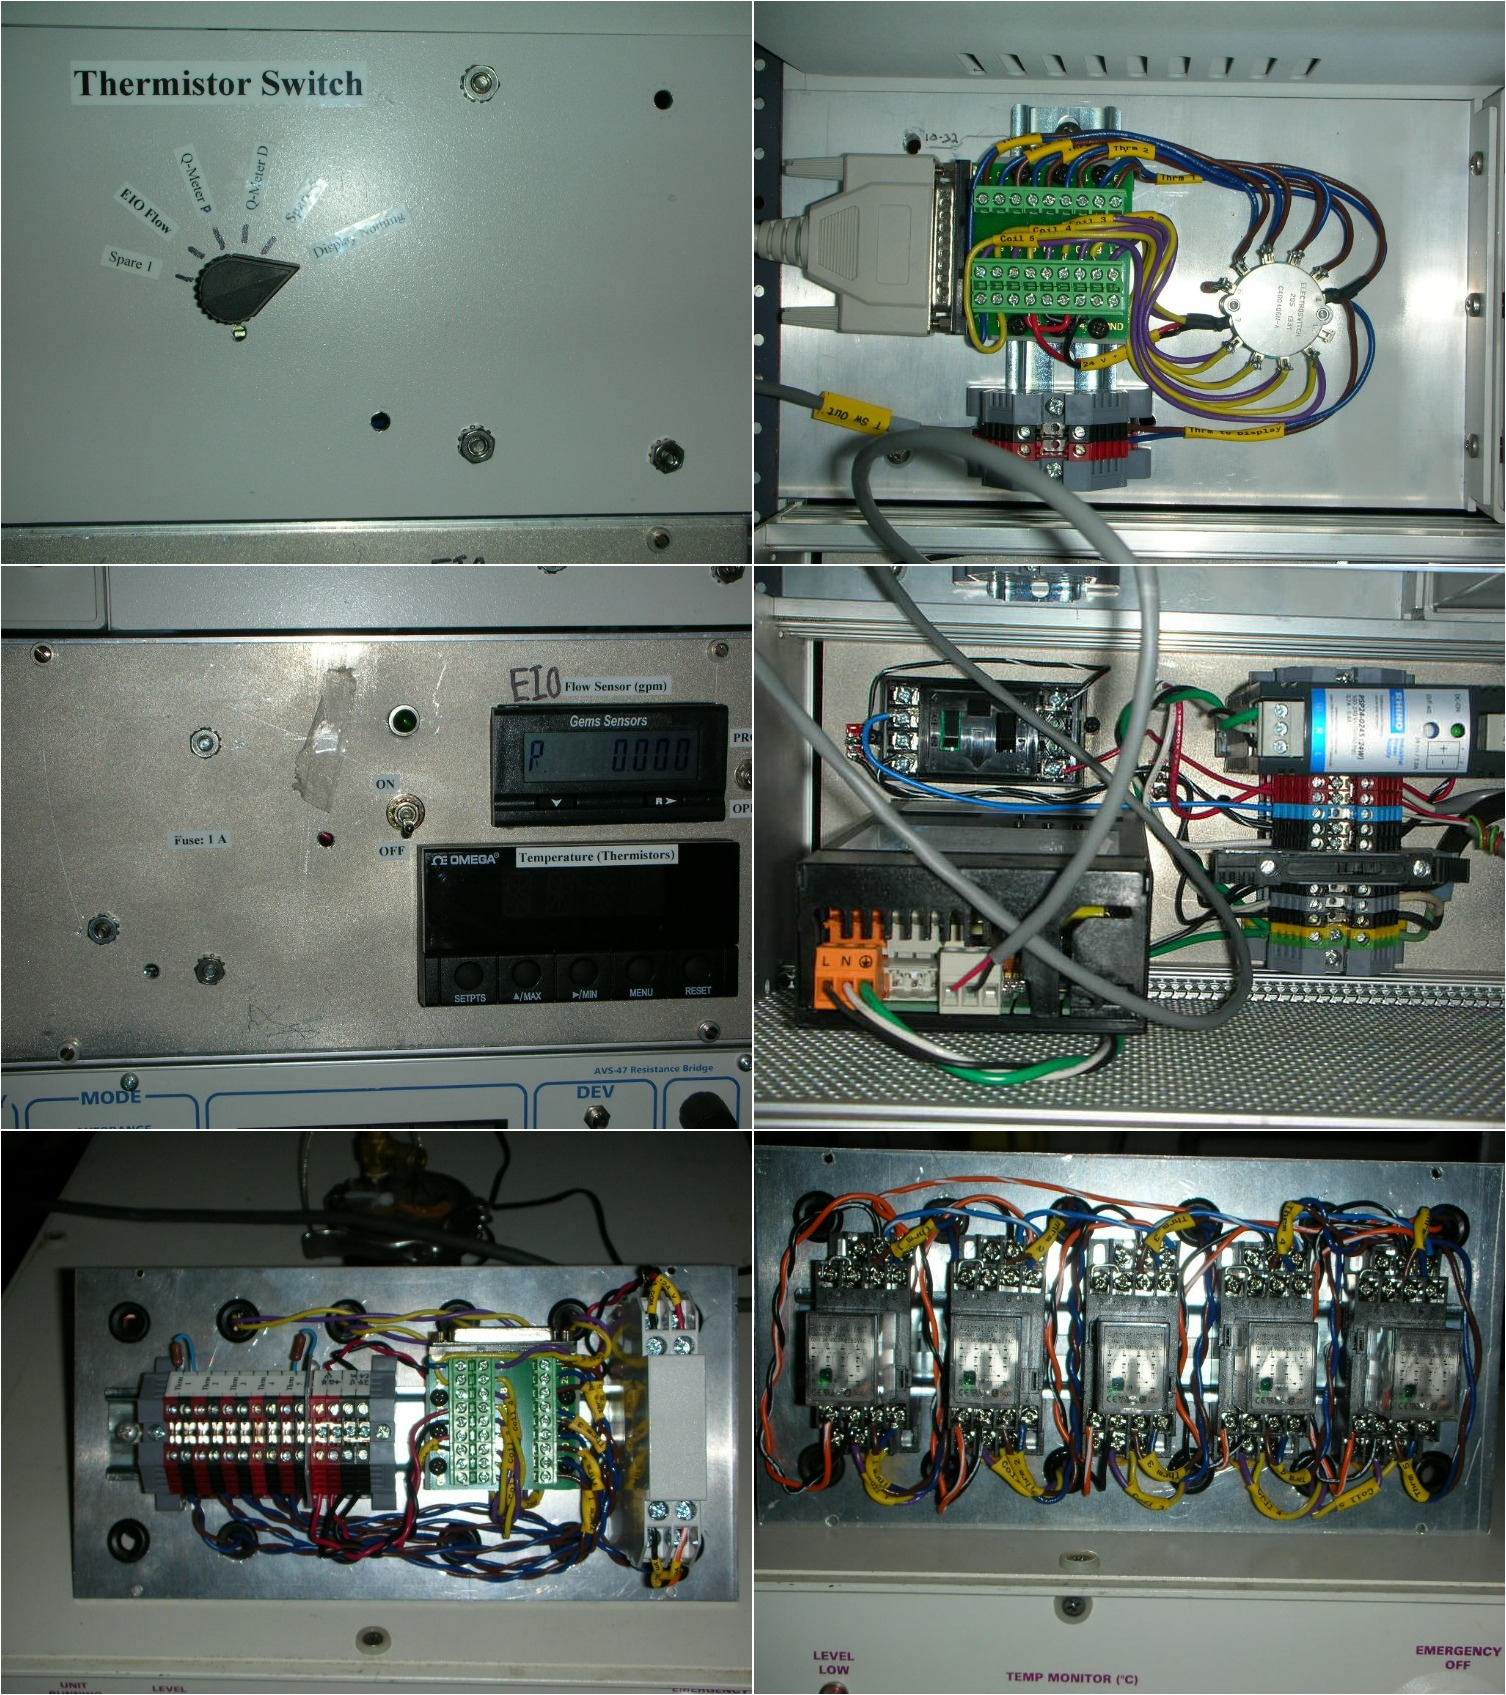
\includegraphics[width=\textwidth]{./img/subsystem-thermistor-photos.png}
 % subsystem-thermistor-photos.png: 0x0 pixel, 0dpi, 0.00x0.00 cm, bb=
 \caption{Photos of thermistor system.}
 \label{fig:subsystem-thermistor-photos}
\end{figure}

\section{IVC Manifold}
The IVC manifold, see diagram on Figure \ref{fig:ivc-manifold-diagram}, connects the turbo pump to the IVC connector on the fridge, allows flow of helium gas during MC cooling, and hosts the Pirani pressure gauge.

\begin{figure}[htbp!]
 \centering
 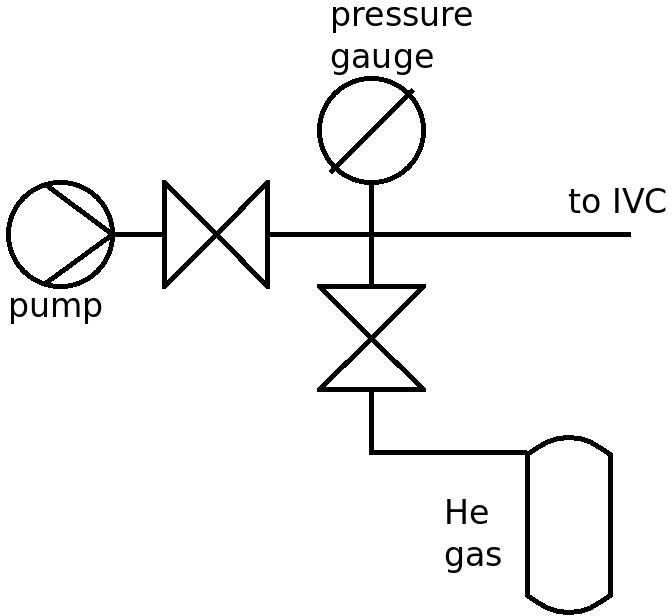
\includegraphics[width=.5\textwidth]{./img/ivc-manifold-diagram.jpg}
 % ivc-manifold-diagram.jpg: 0x0 pixel, 0dpi, 0.00x0.00 cm, bb=
 \caption{The IVC turbo and mechanical pumps evacuate the manifold and IVC line.  The gas line is used to backfill the IVC to about 40 mbar, measured with the pressure gauge, of exchange gas during cooling.}
 \label{fig:ivc-manifold-diagram}
\end{figure}

The pump cart the IVC sits on is powered by first plugging in the turbo pump fan, then plugging in the turbo pump controller, and finally, plugging in the mechanical pump, which automatically starts it up.

\section{OVC Manifold}
The OVC manifold is simply a valve on top of a turbo pump that connects to the OVC pump out ports on the fridge.  Between the fridge and the valve is a tee with a cold cathode pressure gauge.  See Figure \ref{fig:ovc-manifold-diagram}.



The green button on the front of the HiCube powers on the controller, and then the power button the front panel starts the pump.  Make sure the ballast valve in the back is closed before pumping.  If the turbo stalls before reaching 1500 Hz, slowly wind down the pump, blank it off, and try again.  Power cycle as a last resort.

\begin{figure}[htbp!]
 \centering
 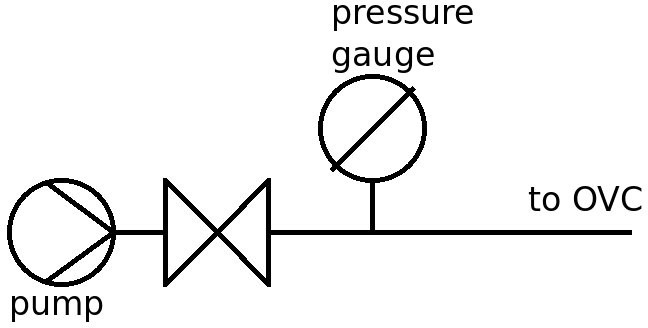
\includegraphics[width=.5\textwidth]{./img/ovc-manifold-diagram.jpg}
 % ovc-manifold-diagram.jpg: 0x0 pixel, 0dpi, 0.00x0.00 cm, bb=
 \caption{The OVC pump is a Pfeiffer HiCube station, and the pressure gauge is a Pfeiffer IKR 251 cold cathode gauge.}
 \label{fig:ovc-manifold-diagram}
 
 
\end{figure}


%-----appendices
\begin{appendices}
\noappendicestocpagenum
\addappheadtotoc
\chapter{Checklist for cooldown}
%-----appendices
\label{appendix:checklist-for-cooldown}

The preparation for a cooldown is not optional.  The checklist in Figure \ref{fig:checklist} should be gone through and double checked before LHe is ordered.


The entire group should be made aware if something on the checklist is not satisfied when LHe is ordered.  All subsequent procedures and operations in the Practical Operation (Chapter \ref{chapter:practical-op}) then need to be reviewed for potential modification to accommodate the missing prep.

\begin{figure}[!htbp]
 \centering
 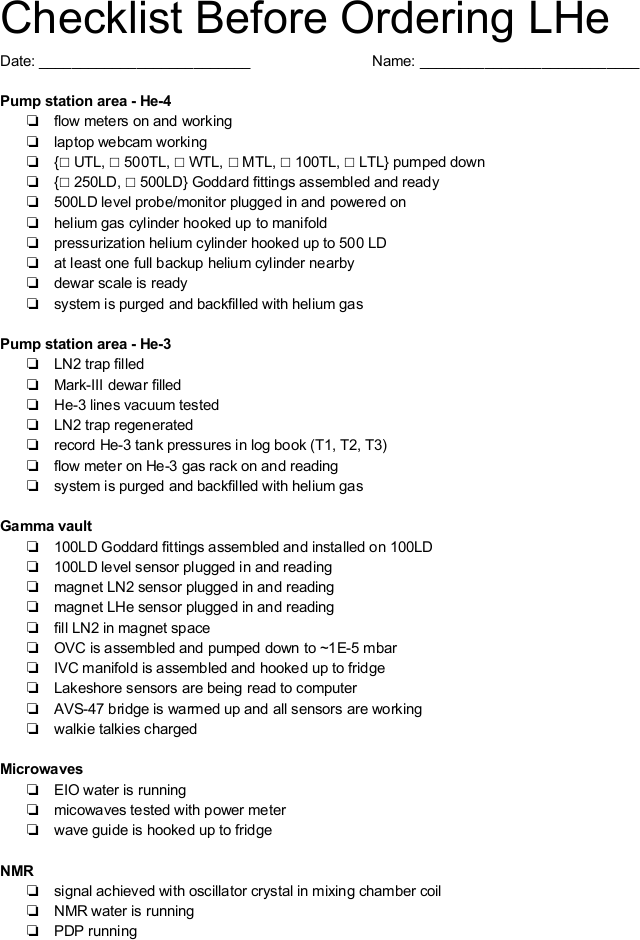
\includegraphics[height=.95\textheight]{./docs/cooldown-checklist.png}
 % cooldown-checklist.pdf: 0x0 pixel, 0dpi, 0.00x0.00 cm, bb=
 \caption{Checklist.}
 \label{fig:checklist}
\end{figure}



\chapter{SLPM Conversion}
\label{appendix:slpm-conversion}
Some HiFrost documents from CERN refer to flow rates of \hef{} and \het{} in millimoles per second.  The formula to convert this flow rate to SLPM is
\begin{equation}
 \textrm{[SLPM]}=\left(\frac{60\textrm{ s}}{\textrm{min}}\right)\left(\frac{x\textrm{ mol}}{\textrm{s}}\right)\left(\frac{4\textrm{ g}}{\textrm{mol}}\right)\left(\frac{1\textrm{ L}}{0.1785\textrm{ g}}\right)
\end{equation}
for \hef{} and 

\begin{equation}
 \textrm{[SLPM]}=\left(\frac{60\textrm{ s}}{\textrm{min}}\right)\left(\frac{x\textrm{ mol}}{\textrm{s}}\right)\left(\frac{3.01\textrm{ g}}{\textrm{mol}}\right)\left(\frac{1\textrm{ L}}{0.135\textrm{ g}}\right)
\end{equation}
for \het{}\cite{linde-helium-3-sheet}, where [SLPM] is the standard flow volume, $x$ is the flow rate in mol/s, $k$ is the Boltzmann constant and the definitions for STP are a temperature of 273.15 K and a pressure of 100 kPa.

Figure \ref{fig:slpm-conversion} shows some values of SLPM to mmol/s flow.

\begin{figure}
\begin{tabular}{|c|c|c|}
\hline
 SLPM& mmol/s (\het)& mmol/s (\hef)\\
\hline
5&3.74&3.71\\
\hline
10&7.48&7.44\\
\hline
15&11.21&11.16\\
\hline
20&14.95&14.86\\
\hline
25&18.69&18.60\\
\hline
30&22.42&22.31\\
\hline
40&29.90&29.75\\
\hline
50&37.38&37.19\\
\hline
60&44.85&44.63\\
\hline
80&59.80&59.50\\
\hline
100&74.75&74.38\\
\hline

\end{tabular}
\caption{Flow rate conversion between mmol/s to SLPM for helium.}
\label{fig:slpm-conversion}
\end{figure} 

\chapter{Transfer Line Drawings}
\label{appendix:tl-drawings}

\begin{figure}[!h]
 \centering
 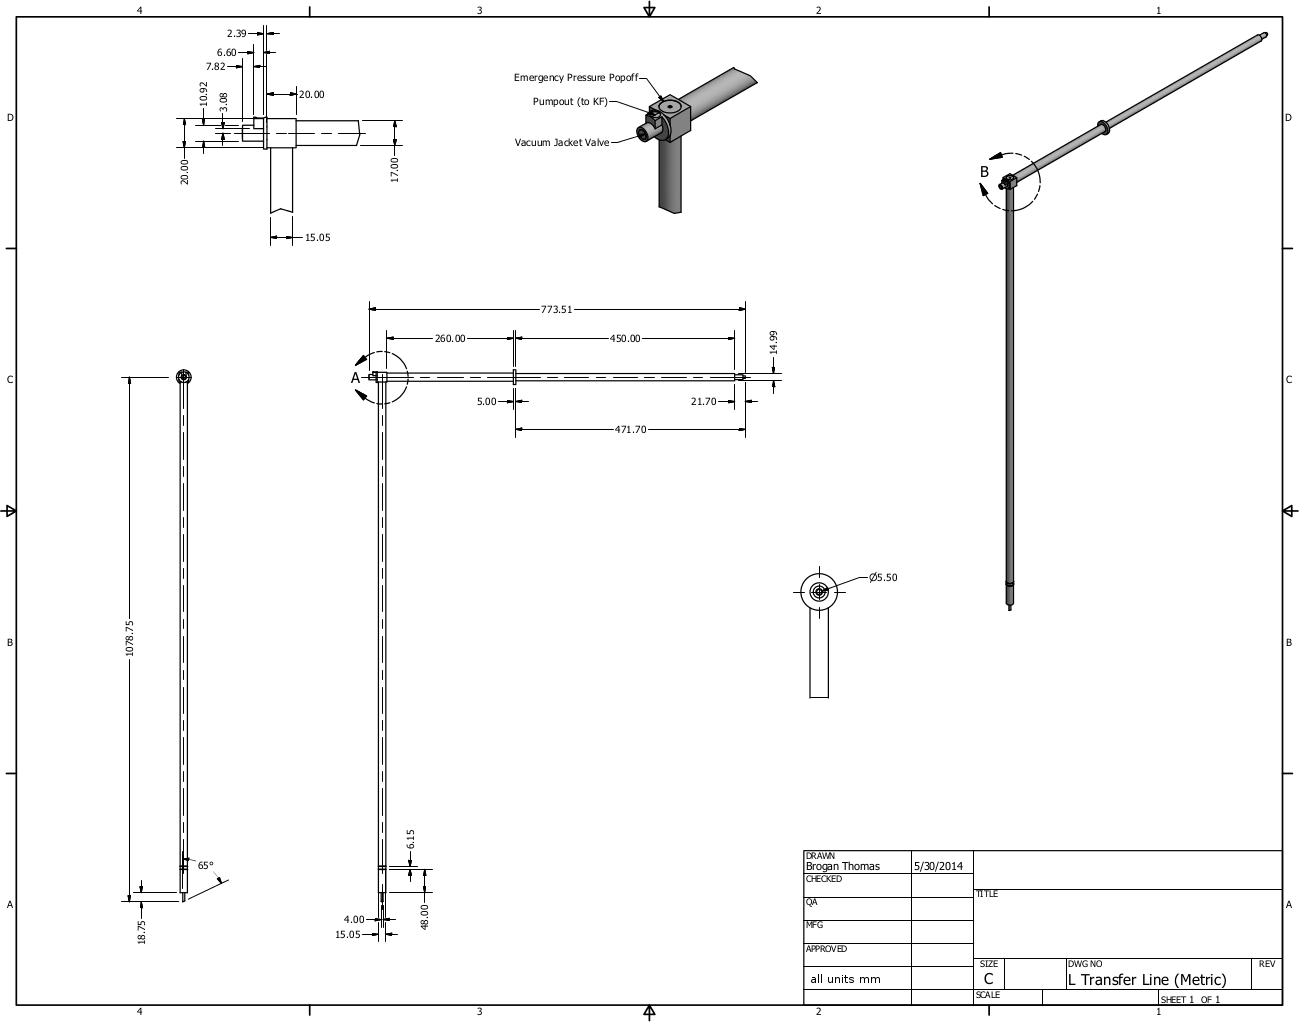
\includegraphics[width=\textwidth]{./img/LTL-drawing.png}
 \caption{Drawing of the LTL.}
 \label{fig:LTL-drawing}
\end{figure}

\begin{figure}[tbp!]
 \centering
 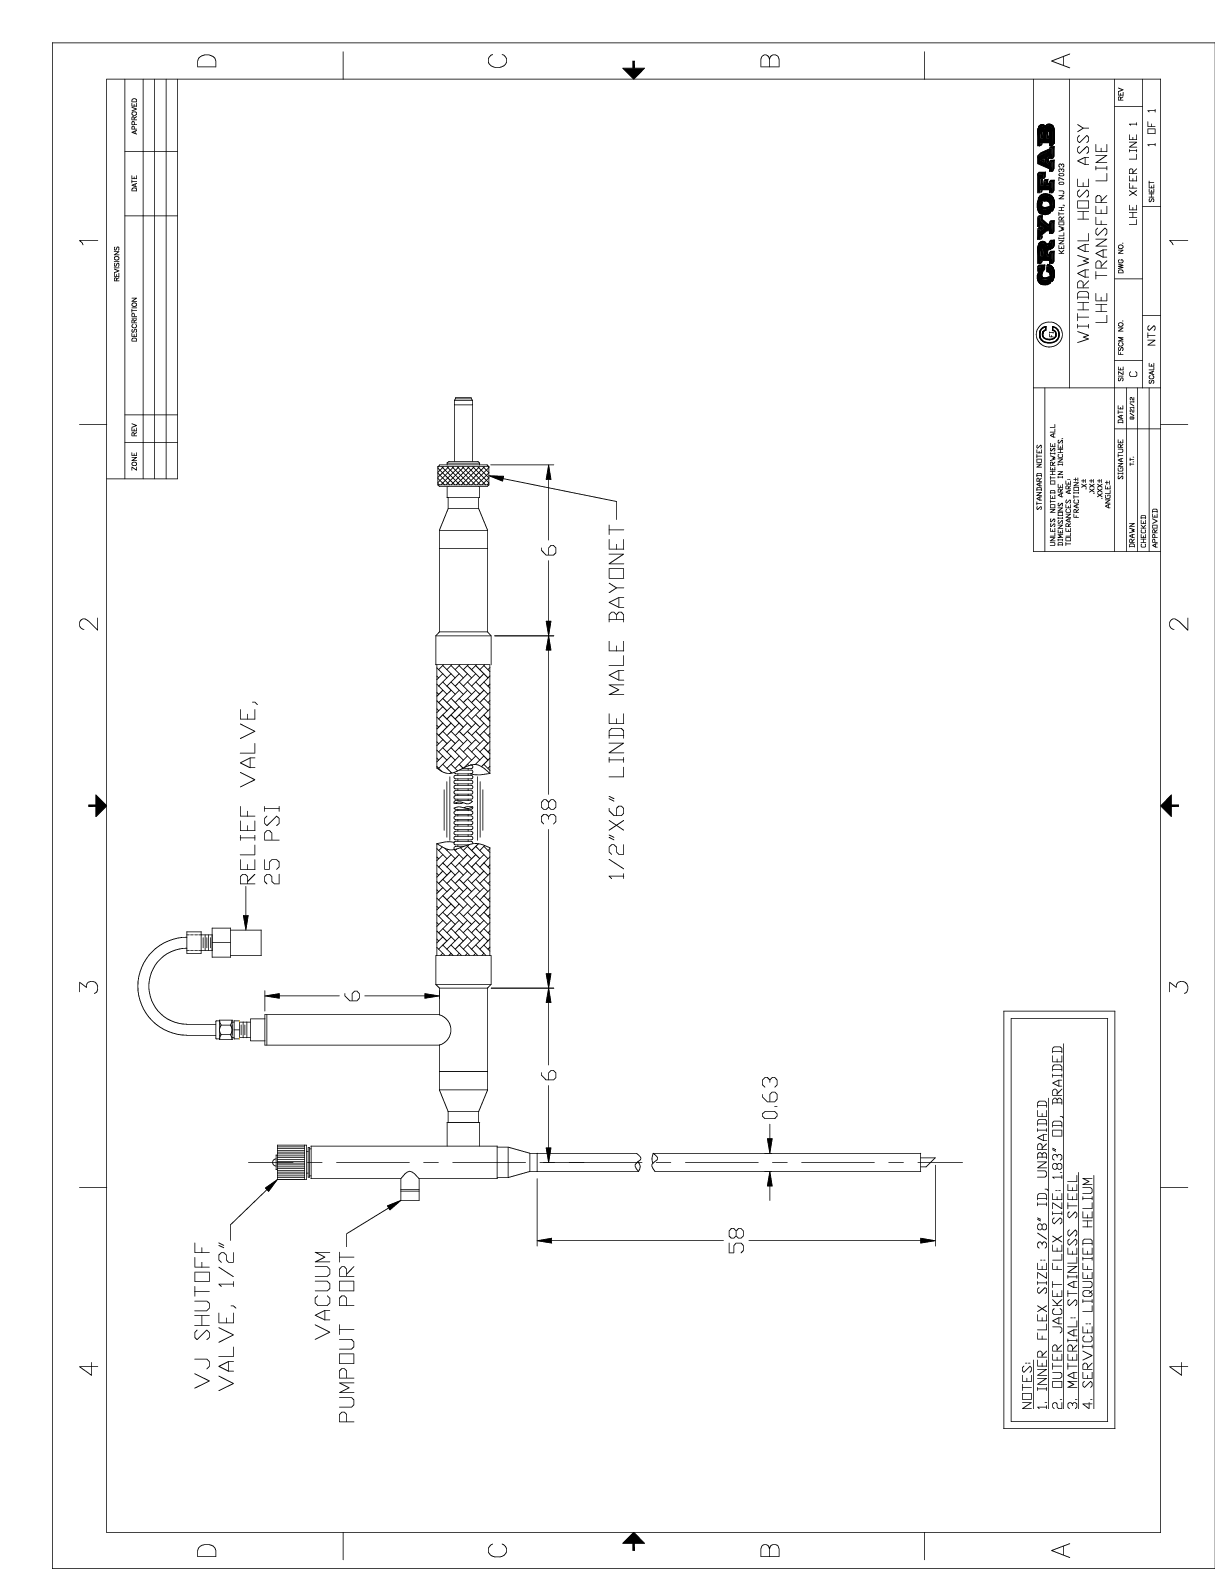
\includegraphics[width=\textwidth]{./img/500TL-drawing.png}
 \caption{Drawing of the 500TL.}
 \label{fig:500TL-drawing}
\end{figure}

\begin{figure}[tbp!]
 \centering
 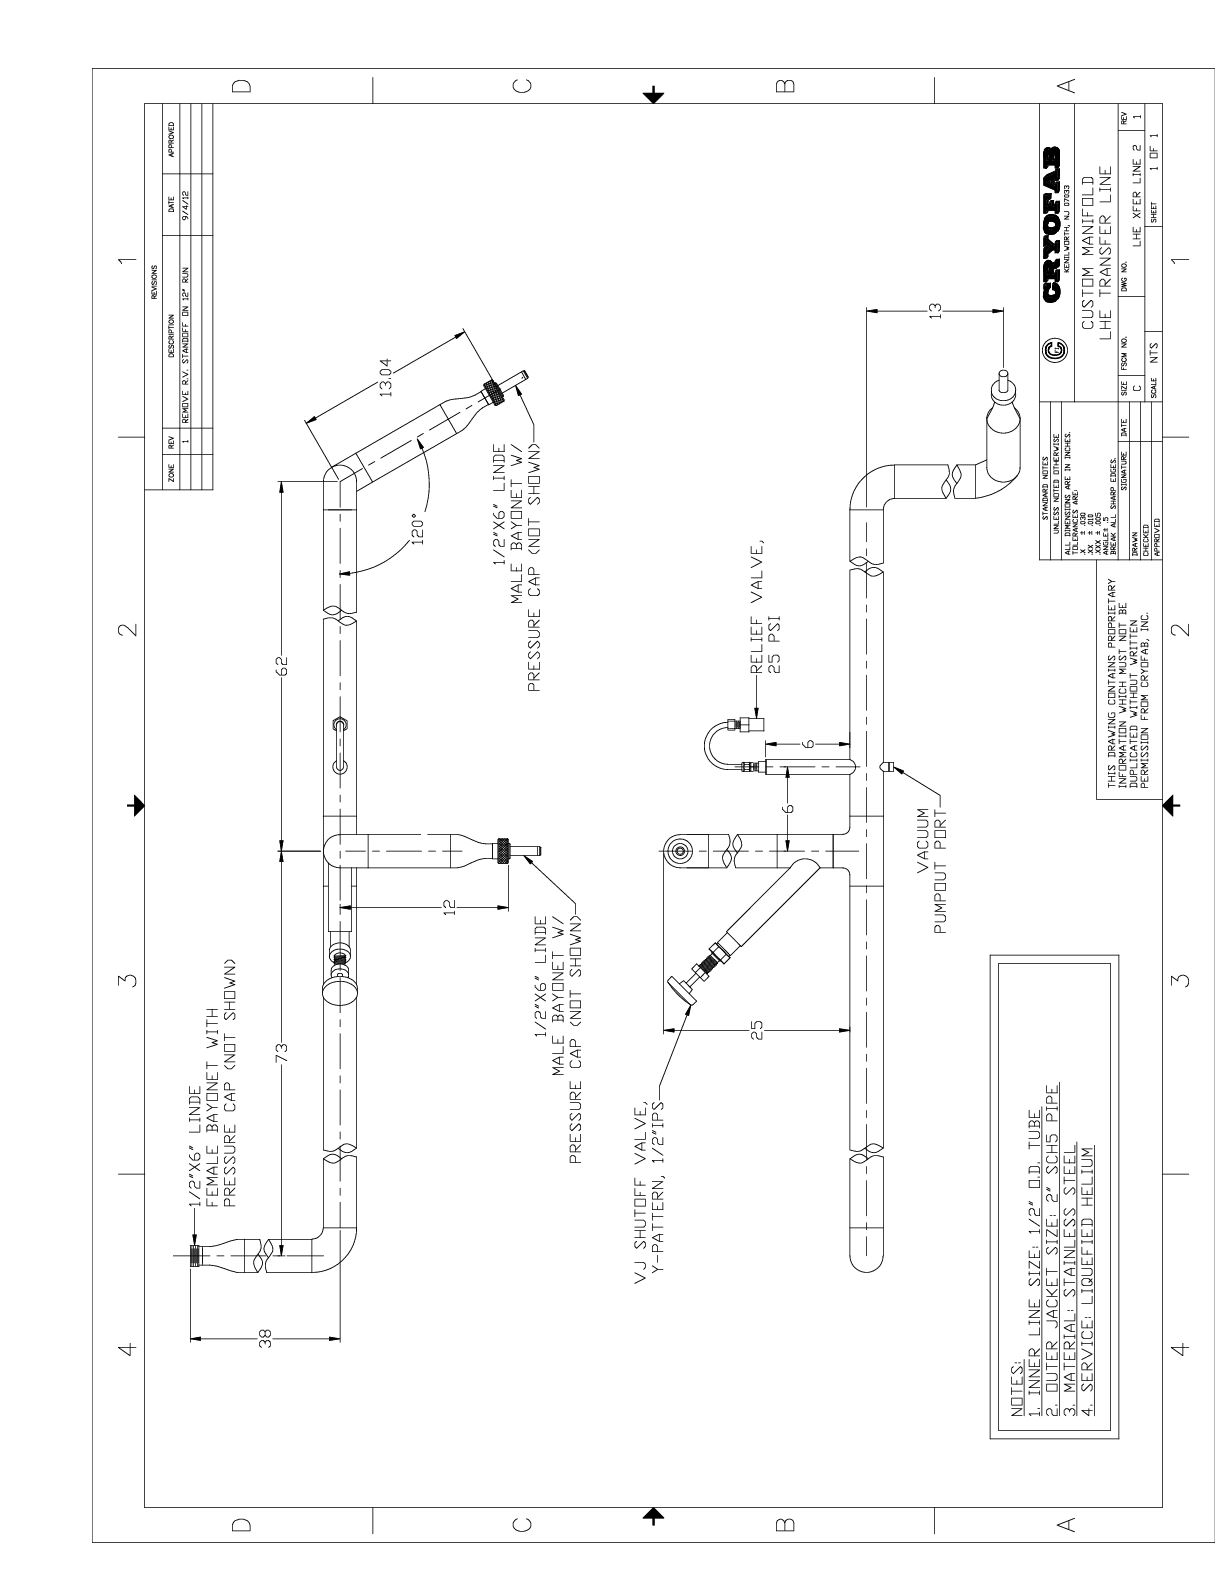
\includegraphics[width=\textwidth]{./img/WTL-drawing.png}
 \caption{Drawing of the WTL.}
 \label{fig:WTL-drawing}
\end{figure}

\begin{figure}[tbp!]
 \centering
 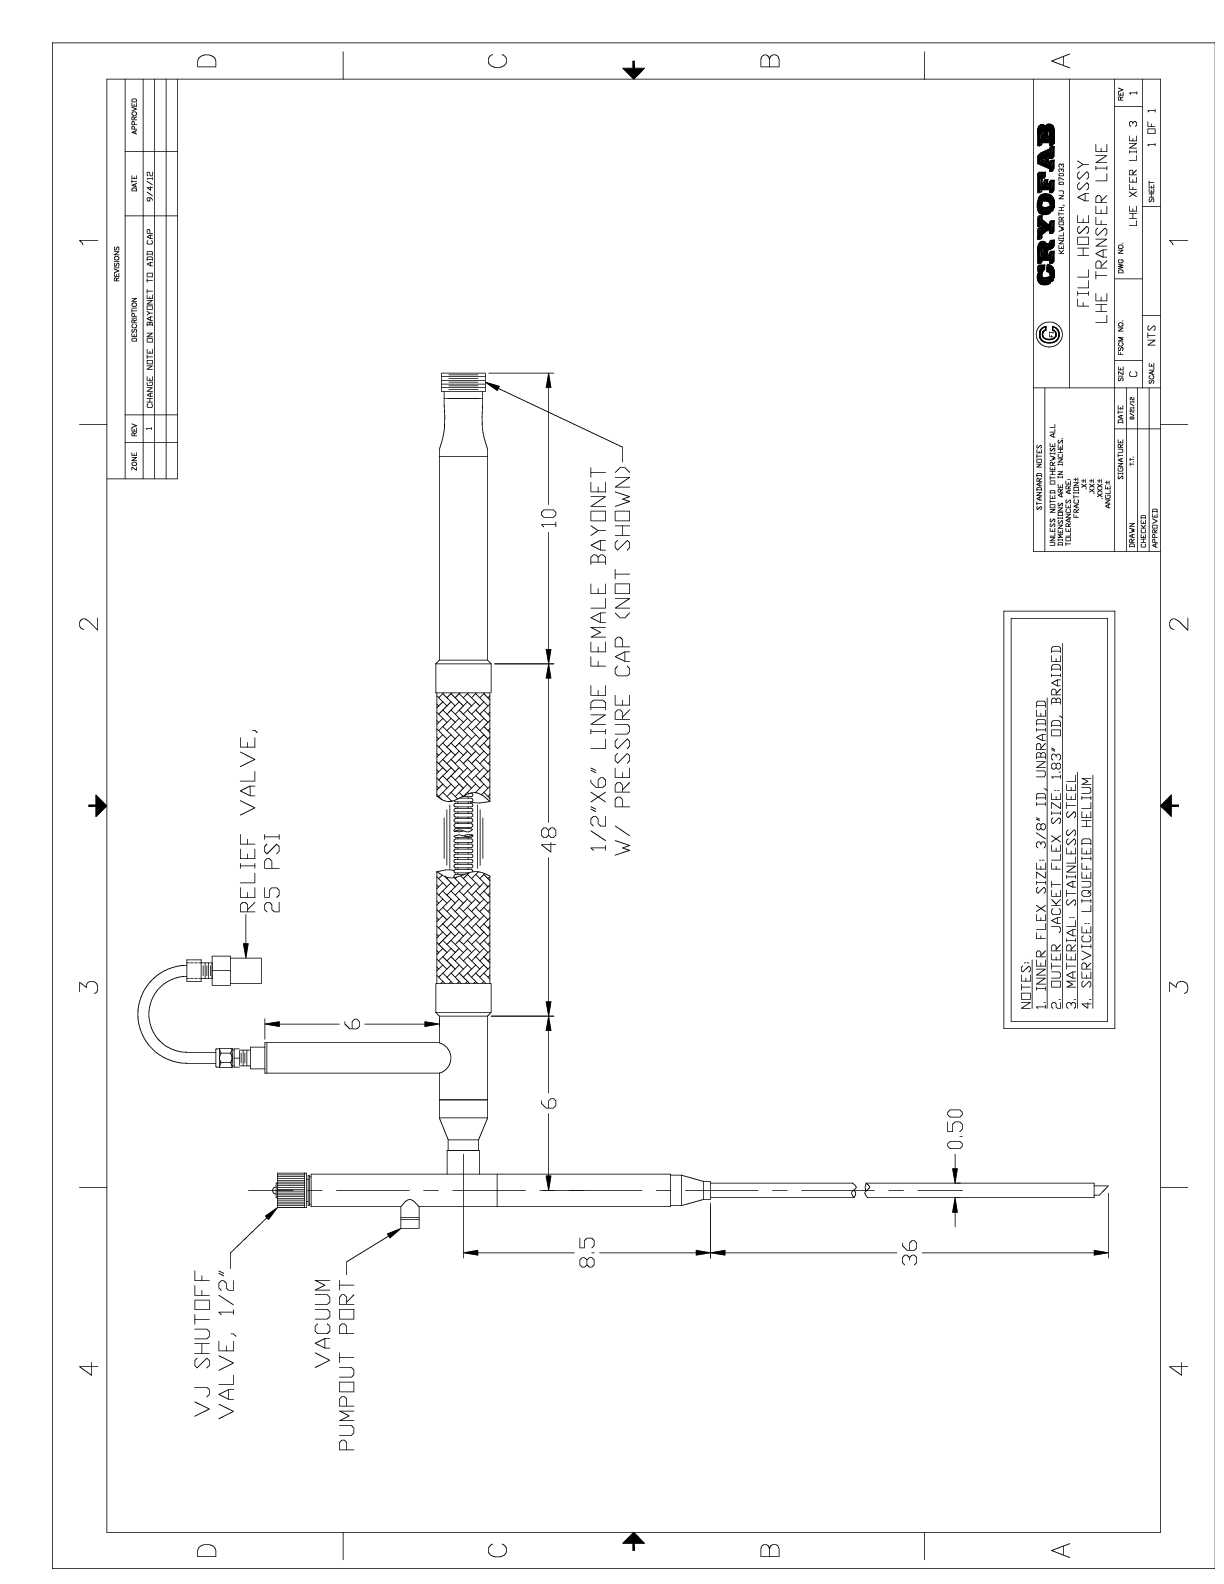
\includegraphics[width=\textwidth]{./img/MTL-drawing.png}
 \caption{Drawing of the MTL.}
 \label{fig:MTL-drawing}
\end{figure}

\begin{figure}[tbp!]
 \centering
 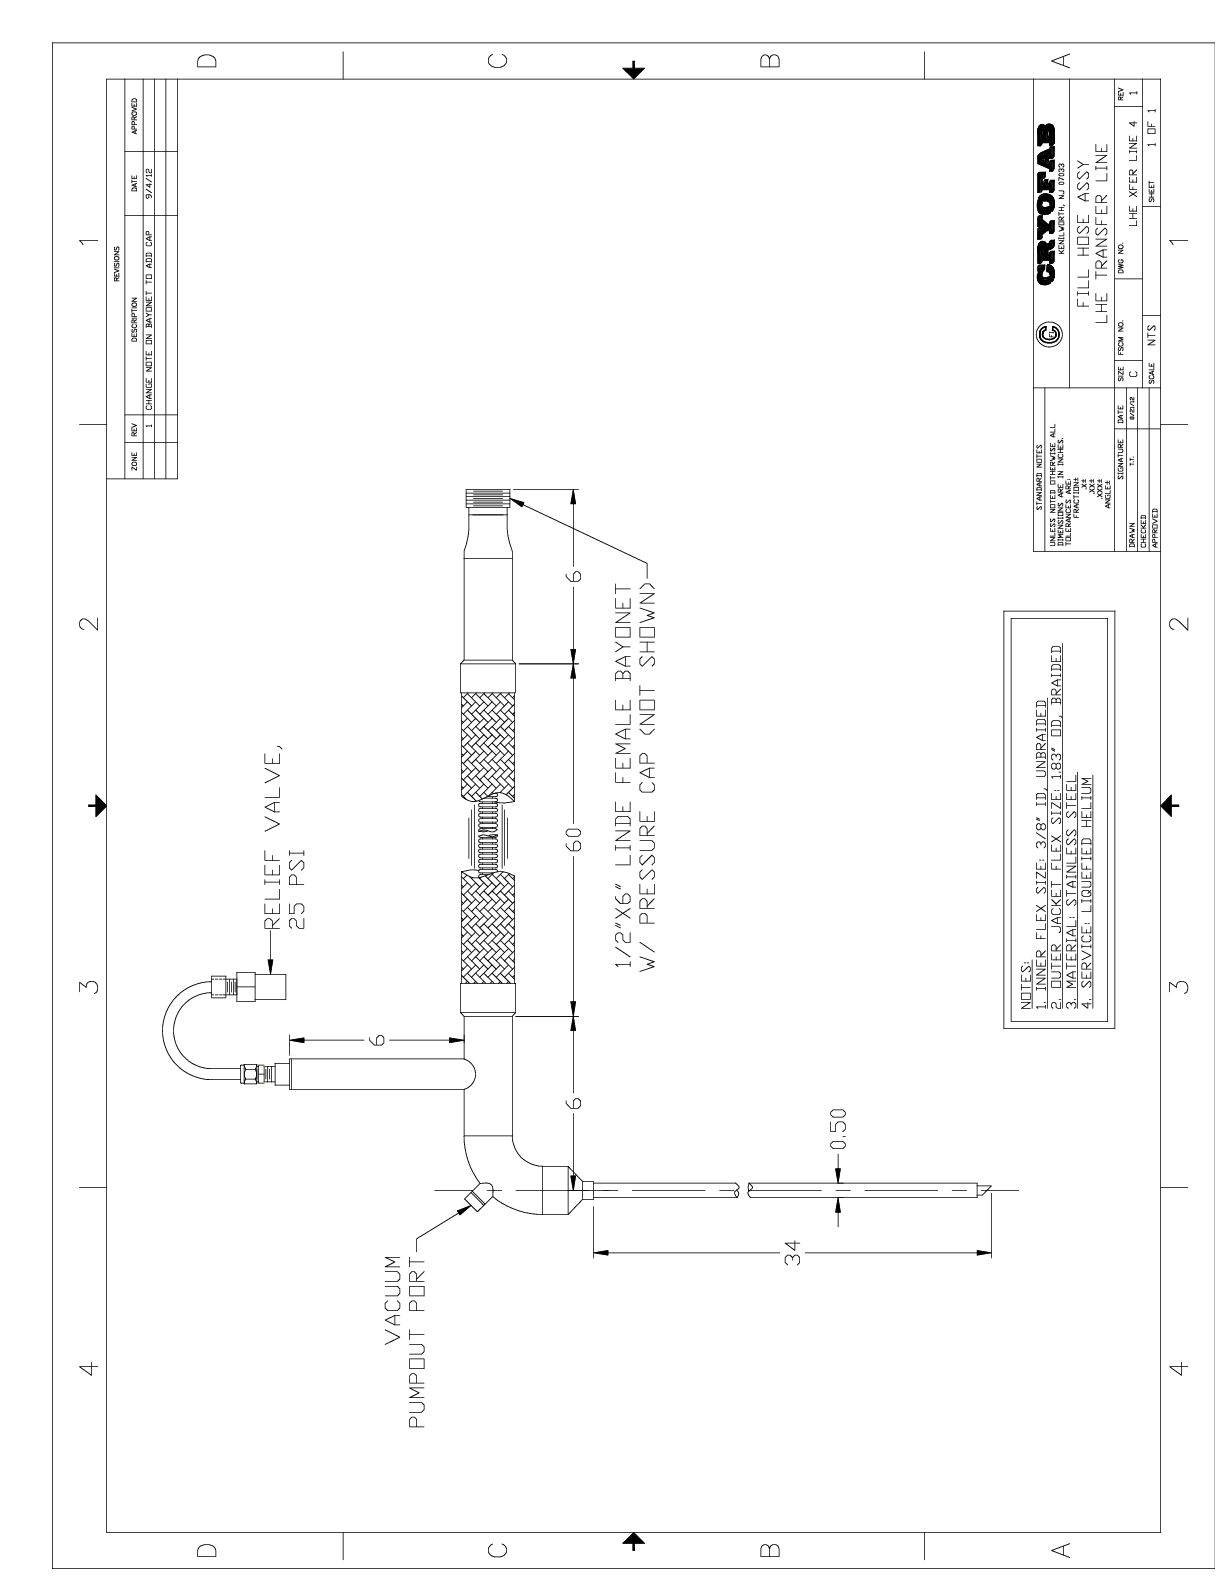
\includegraphics[width=\textwidth]{./img/100TL-drawing.png}
 \caption{Drawing of the 100TL.}
 \label{fig:100TL-drawing}
\end{figure}
\end{appendices}
%-----appendices
%\begin{appendices}
%\noappendicestocpagenum
%\addappheadtotoc
%\chapter{Checklist for cooldown}
%-----appendices
%\appendix
%\label{appendix}
%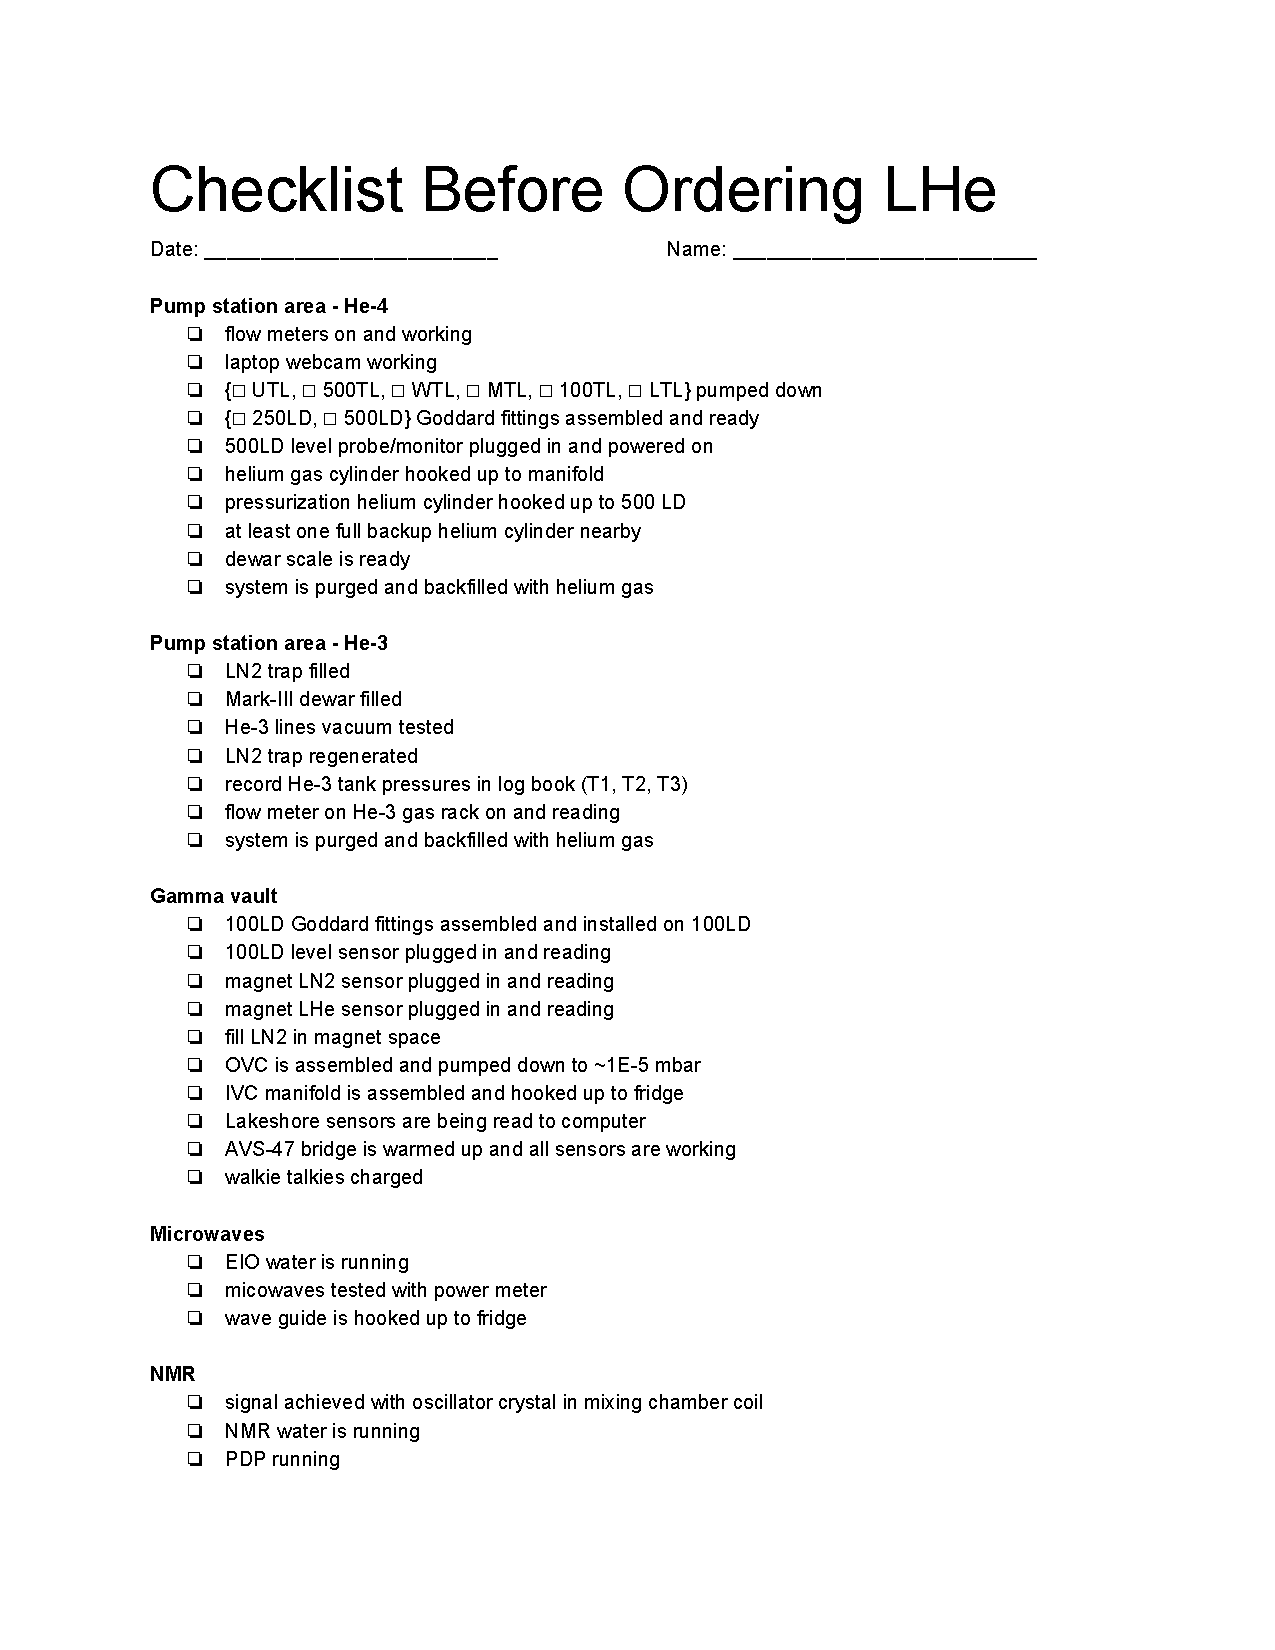
\includepdf[pages={1}]{docs/cooldown-checklist.pdf}
%\end{appendices}

\backmatter 


%\include{glossary} 
%\include{notat} 
\bibliographystyle{amsalpha} %The style you want to use for references. 
\bibliography{refs.bib} %The files containing all the articles and books you ever referenced. 
%\printindex %Make an index AUTOMATICALLY 

\end{document}
